\documentclass{article}

\usepackage{csquotes}
% 使用中文CJK包
\usepackage{CJK}
% 图像插入宏包
\usepackage{graphicx}
% 自定义颜色支持
\usepackage[usenames,dvipsnames]{color}
% 长表格跨页支持
\usepackage{longtable}
% 代码高亮支持
\usepackage{listings}
% 算法伪代码包
\usepackage[ruled,vlined]{algorithm2e}
% 自定义标题格式
\usepackage{titlesec}
% 扩展tabular样式
\usepackage{array}
% 添加页眉页脚
\usepackage{fancyhdr}
% 虚拟正文测试
\usepackage{lipsum}
% 数学环境包
\usepackage{amsmath}
% 首行缩进
\usepackage{indentfirst}
% 树状结构图
\usepackage{tree-dvips}
% 脚注环境
\usepackage{footnote}
% 定制表格线
\usepackage{makecell}
% tikz绘图包
\usepackage{tikz}
% URL超链接
\usepackage[dvips, colorlinks, linkcolor=black]{hyperref}
% 断行URL超链接
\usepackage{breakurl}


% hyperref中文兼容
\pdfstringdefDisableCommands{
\let\CJK@XX\relax
\let\CJK@XXX\relax
\let\CJK@XXXp\relax
\let\CJK@XXXX\relax
\let\CJK@XXXXp\relax
}

\usetikzlibrary{positioning,shapes,shadows,arrows}


% 设置脚注在table中可用
\makesavenoteenv{table}

% 设置标题格式
%\titleformat{\chapter}{\raggedright\Huge\bfseries}{Chapter \thechapter}{1em}{}

% 设置默认字体族, 具体字体请查看texdoc psnfss2e

% 设置Roman字体为Palatino
\renewcommand{\rmdefault}{ppl} 
% 设置TypeWriter字体为Courier
\renewcommand{\ttdefault}{pcr} 

% 设置行距
\setlength{\parskip}{1ex}

% 定义需要的颜色

\definecolor{lightgray}{RGB}{230,230,230}
\definecolor{lightblue}{RGB}{224, 224, 255}
\definecolor{darkblue}{RGB}{192, 192, 255}
\definecolor{lightpink}{RGB}{255, 224, 224}
\definecolor{darkpink}{RGB}{255, 192, 192}
\definecolor{keywordyellow}{RGB}{255, 204, 0}
\definecolor{keywordred}{RGB}{194, 58, 0}
\definecolor{numbercolor}{RGB}{102, 51, 0}

% 设置代码风格

% 定义makefile代码风格
\lstdefinestyle{mcode}
{ 
    language=make, 
    numbers=left, 
    numberstyle=\color{numbercolor},
    basicstyle=\scriptsize\ttfamily\bfseries,
    keywordstyle=\color{blue}, 
    commentstyle=\color{PineGreen},
    stringstyle=\color{red}, 
    frame=shadowbox, 
    frameround=tttt,
    breaklines=true,
    backgroundcolor=\color{lightgray} }
    
% 定义C语言代码风格
\lstdefinestyle{ccode}
{ 
    language=C, 
    numbers=left, 
    numberstyle=\color{numbercolor},
    basicstyle=\scriptsize\ttfamily\bfseries,
    keywordstyle=\color{blue}, 
    commentstyle=\color{PineGreen},
    stringstyle=\color{red}, 
    frame=shadowbox, 
    frameround=tttt,
    breaklines=true,
    backgroundcolor=\color{lightgray} }

% 定义汇编语言代码风格
\lstdefinestyle{acode}
{ 
    language=,
    morekeywords=[1]{mov, movl, movb, movw, orl, xorw, cli, cld, inb, testb, test, jnz, push, pop, jmp, call, lea, add, sub, ret, jle, outb, ljmp, lgdt, cmp, jne, popal, int, jns, pushw, pushal, pushl, popfl, addl, subl},
    morekeywords=[2]{ax, bx, cx, dx, eax, ebx, ecx, edx, cr0, cr1, cr2, cr3, al, ds, es, ss, esp, ebp, esi, edi}, 
    morekeywords=[3]{data, text, bss},
    morekeywords=[4]{long, align, p2align, ascii, fill, globl, space, set, rept, byte, word},
    morecomment=[l]\#,
    numbers=left, 
    numberstyle=\color{numbercolor},
    basicstyle=\scriptsize\ttfamily\bfseries,
    keywordstyle=[1]\color{blue}, 
    keywordstyle=[2]\color{keywordyellow},
    keywordstyle=[3]\color{orange},
    keywordstyle=[4]\color{keywordred},
    commentstyle=\color{PineGreen},
    stringstyle=\color{red}, 
    frame=shadowbox, 
    frameround=tttt,
    breaklines=true,
    backgroundcolor=\color{lightgray} }

    
% 定义命令行输出风格
\lstdefinestyle{console}
{
    language=bash, 
    numbers=none, 
    frame=tRBl,
    basicstyle=\scriptsize\color{green}\ttfamily\bfseries,     
    backgroundcolor=\color{black}}


% 定义exercise输出风格
\lstdefinestyle{exercise}
{
    numbers=none, 
    frame=tRBl,
    breaklines=true,
    breakindent=0pt,
    framexleftmargin=1em,
    framexrightmargin=1em,
    framextopmargin=2ex,
    framexbottommargin=2ex,
    xleftmargin=0.05\linewidth,
    xrightmargin=0.05\linewidth,
    basicstyle=\scriptsize\ttfamily\mdseries,   
    moredelim=[is][\ttfamily\bfseries]{|}{|},
    framerule=0.8pt,
    rulecolor=\color{darkblue}, 
    backgroundcolor=\color{lightblue}}
    

% 定义challenge输出风格
\lstdefinestyle{challenge}
{
    numbers=none, 
    frame=tRBl,
    breaklines=true,
    breakindent=0pt,
    framexleftmargin=1em,
    framexrightmargin=1em,
    framextopmargin=2ex,
    framexbottommargin=2ex,
    xleftmargin=0.05\linewidth,
    xrightmargin=0.05\linewidth,
    basicstyle=\scriptsize\ttfamily\mdseries,   
    moredelim=[is][\ttfamily\bfseries]{|}{|},
    framerule=0.8pt,
    rulecolor=\color{darkpink}, 
    backgroundcolor=\color{lightpink}}
    


% 非常重要, listings关闭非ASCII字符兼容
\lstset{extendedchars=false}


% 定义问题的答案格式
\newcommand{\highlight}[1]{{\bfseries \color{red}  #1}}
% 定义函数名格式
\newcommand{\funcname}[1]{{\ttfamily \small #1}}




\pagestyle{fancy}
\begin{document}
\begin{CJK*}{UTF8}{gkai}

\lhead{操作系统实习报告}
\rhead{张弛, 00848231}
\title{操作系统JOS实习第六次报告}
\author{张弛 \hspace{1ex} 00848231, \\
        zhangchitc@gmail.com}

\maketitle
% 记得在文档末尾插入\clearpage
\tableofcontents
\newpage

\section{Introduction}

此次Lab是所有JOS实验中最恶心的一次,需要阅读的东西超过了以前所有的总和。所以请做好准备。

在真正下手之前,最好的话请完整的将MIT的材料完整的读一遍,对各个名词和部分有个大致的印象。其他要读的材料还有很多,具体的部分我在报告中会着重提到。


纵观全局,这次Lab的最大难点就是在于你需要\highlight{从零开始}写出一个E100网卡的驱动程序。这个驱动程序从Web Server接收IPC调用向网卡发送数据,然后从网卡接收数据发回给Web Server。这和我们以前的实验都不一样,以前都是给出了结构的框架,我们只需要针对一个具体的功能函数进行细节的填补即可,相关的数据结构、接口设置都为我们设计好了。这次需要我们从头到尾完成整个网卡驱动,困难可想而知。

除开网卡之外的部分都相对简单。因此我们这篇报告重点介绍如何完成这个网卡驱动。操纵网卡我们需要了解的方面有:

\begin{enumerate}
\item{一个PCI设备在JOS中的设置和相关数据结构}
\item{扫描和初始化网卡}
\item{网卡的关键结构}
\item{网卡如何和操作系统交互数据}
\item{如何对网卡发送指令}
\end{enumerate}

报告在后面会一步一步从课程给出的资料中抽取出这些细节。同时我在写的过程中参考了\burl{http://code.google.com/p/os-xv6-network}项目主页提供的一份源代码,说的比较极端的话我基本是完全照搬了它的代码,不过这并不影响,学习别人优秀的代码本来就是编程中获得提高最有效的方式。重要的仍是个人的理解。


\section{Initialization and transmitting packets}

对于Network Server的架构,我们只需要大致了解模块即可,这次的实验很少需要对Server进行大规模的修改。

\subsubsection{The Timer Environment}

\begin{lstlisting}[style=exercise]
|Exercise 1|. Add a call to time_tick for every clock interrupt in kern/trap.c. Implement sys_time_msec and add it to syscall in kern/syscall.c so that user space has access to the time.
\end{lstlisting}

这个Exercise太简单了就不贴代码了,唯一需要注意的是在测试用户程序testtime之前由于我们还没有实现网络服务器的部分,所以需要注释掉JOS载入网络服务器的部分:

\begin{lstlisting}[style=ccode, title={\scriptsize \ttfamily \bfseries kern/init.c: i386\_init()}]
	// Should always have an idle process as first one.
	ENV_CREATE(user_idle);

	// Start fs.
	ENV_CREATE(fs_fs);

#if !defined(TEST_NO_NS)
	// Start ns.
	//ENV_CREATE(net_ns);
#endif
\end{lstlisting}

这样运行客户程序才不会出错。


\subsubsection{The Output Environment}

\label{outputhelp}

\subsubsection{The Input Environment}

这两部分在材料中也提到了我们需要先实现驱动程序和系统调用部分才可以完成。所以我们先放下他们关注最重要的驱动部分。

\subsection{The Network Interface Card}


\begin{lstlisting}[style=exercise]
|Exercise 2|. Browse the Intel 82559 page and look at these two documents:

    1. Intel 8255x 10/100 Mbps Ethernet Controller Family Open Source Software Developer Manual (local copy)
    2. 82559ER Fast Ethernet PCI Controller Datasheet (local copy)

Do not worry about the details in your first pass. It is more important to read this assignment write-up first to get a high level pictures of how the Intel chip is organized and what is needed to create a device driver.

When you do read the open source developer manual in depth, glance over Section 4 to learn about the PCI interface but pay very close attention to Section 6 as it deals with the Software Interface. In fact, most everything you need is in Section 6. Use the datasheet solely as a reference if you find the developer manual vague.

A simple E100 driver needs only a fraction of the features and interfaces that the card provides. When you're reading through the developer manual, think carefully about the easiest way to interface with the card. You're of course welcome to use its more advanced, high-performance features (in fact, some of the challenge exercises ask you to do exactly this), but it's a good idea to get a basic driver working first.

The acronyms in both documents can get overwhelming. Consult the glossary at the end of this lab assignment for some help.
\end{lstlisting}


打开资料是不是已经晕了?这是我觉得这个Lab设计的非常不好的原因之一,一开始就甩出一大堆手册要我们看,而不是给出一个纵览性的结构和指南。先放下吧,后面我们再慢慢说具体要看这些资料的哪些部分。


\subsubsection{PCI Interface}

在使用网卡之前,我们先要通知硬件系统扫描出所有的PCI设备,并且找出其中的E100网卡,对其进行初始化。这是这部分任务的最终目的,为我们操作网卡做好准备工作。这里我们将大致介绍一下PCI设备的一些基础知识:

\begin{description}
\item[什么是PCI设备]:\\

PCI是外围设备互连(Peripheral Component Interconnect)的简称,是在目前的计算机系统中得到了非常广泛应用的通用总线接口标准。

\begin{itemize}
\item{在一个PCI系统中,最多可以有256根PCI总线,一般的主机上只会用到其中很少的几条,比如Bus 0和Bus 1。}
\item{在一根PCI总线上可以连接多个物理设备,可以是一个网卡、显卡声卡等等。最多不超过32个。一般来说因为物理特性的限制,一条总线上不会有太多的设备。}
\item{一个PCI物理设备可以有多个功能,比如同时提供视频解析和声音解析。最多提供8个功能。}
\item{每个功能对应一个256 bytes的PCI Configuration Space,这个在我们接下来对网卡进行初始化的时候会特别提到这个东西的。}
\end{itemize}


所以对于一个PCI设备的具体功能,我们可以使用 {\bfseries 总线号:设备号:功能号}来对其进行定位,比如在Ubuntu下我们使用lspci命令,就可以得到这样的输出:

\begin{lstlisting}[style=console, basicstyle=\tiny\color{green}\ttfamily\bfseries]
zhangchi@zhangchi-vostro1400:~$ lspci 
00:00.0 Host bridge: Intel Corporation Mobile PM965/GM965/GL960 Memory Controller Hub (rev 0c)
00:02.0 VGA compatible controller: Intel Corporation Mobile GM965/GL960 Integrated Graphics Controller (rev 0c)
00:02.1 Display controller: Intel Corporation Mobile GM965/GL960 Integrated Graphics Controller (rev 0c)
00:1a.0 USB Controller: Intel Corporation 82801H (ICH8 Family) USB UHCI Controller #4 (rev 02)
00:1a.1 USB Controller: Intel Corporation 82801H (ICH8 Family) USB UHCI Controller #5 (rev 02)
00:1a.7 USB Controller: Intel Corporation 82801H (ICH8 Family) USB2 EHCI Controller #2 (rev 02)
00:1b.0 Audio device: Intel Corporation 82801H (ICH8 Family) HD Audio Controller (rev 02)
00:1c.0 PCI bridge: Intel Corporation 82801H (ICH8 Family) PCI Express Port 1 (rev 02)
00:1c.1 PCI bridge: Intel Corporation 82801H (ICH8 Family) PCI Express Port 2 (rev 02)
00:1c.3 PCI bridge: Intel Corporation 82801H (ICH8 Family) PCI Express Port 4 (rev 02)
00:1c.5 PCI bridge: Intel Corporation 82801H (ICH8 Family) PCI Express Port 6 (rev 02)
00:1d.0 USB Controller: Intel Corporation 82801H (ICH8 Family) USB UHCI Controller #1 (rev 02)
00:1d.1 USB Controller: Intel Corporation 82801H (ICH8 Family) USB UHCI Controller #2 (rev 02)
00:1d.2 USB Controller: Intel Corporation 82801H (ICH8 Family) USB UHCI Controller #3 (rev 02)
00:1d.7 USB Controller: Intel Corporation 82801H (ICH8 Family) USB2 EHCI Controller #1 (rev 02)
00:1e.0 PCI bridge: Intel Corporation 82801 Mobile PCI Bridge (rev f2)
00:1f.0 ISA bridge: Intel Corporation 82801HEM (ICH8M) LPC Interface Controller (rev 02)
00:1f.1 IDE interface: Intel Corporation 82801HBM/HEM (ICH8M/ICH8M-E) IDE Controller (rev 02)
00:1f.2 IDE interface: Intel Corporation 82801HBM/HEM (ICH8M/ICH8M-E) SATA IDE Controller (rev 02)
00:1f.3 SMBus: Intel Corporation 82801H (ICH8 Family) SMBus Controller (rev 02)
03:01.0 FireWire (IEEE 1394): Ricoh Co Ltd R5C832 IEEE 1394 Controller (rev 05)
03:01.1 SD Host controller: Ricoh Co Ltd R5C822 SD/SDIO/MMC/MS/MSPro Host Adapter (rev 22)
03:01.2 System peripheral: Ricoh Co Ltd R5C843 MMC Host Controller (rev 12)
03:01.3 System peripheral: Ricoh Co Ltd R5C592 Memory Stick Bus Host Adapter (rev 12)
03:01.4 System peripheral: Ricoh Co Ltd xD-Picture Card Controller (rev ff)
09:00.0 Ethernet controller: Broadcom Corporation NetLink BCM5906M Fast Ethernet PCI Express (rev 02)
0c:00.0 Network controller: Intel Corporation PRO/Wireless 3945ABG [Golan] Network Connection (rev 02)
\end{lstlisting}

看到前面用冒号和点分割的数字了么,就是以总线号、设备号以及功能号进行标识的。可以看到我的机器上用到了0、3、9、12这四条PCI总线。

\item[PCI配置寄存器]:\\

每一个PCI设备都有它映射的内存地址空间和它的I/O区域。除此之外,PCI设备还有它的配置寄存器(即Configuration Space)。对于所有的PCI设备,配置地址空间一共256 bytes,其中前64 bytes是标准化的,它提供了厂商号,设备号,版本号等信息,唯一标识一个PCI设备。同时,它也提供了最多可多达6个的I/O地址区域,每个区域可以是内存也可以是I/O地址。这几个I/O地址区域是驱动程序找到设备映射到内存和I/O空间的具体位置的唯一途径。关于这64个字节的配置空间的详细情况,可以参考下图:

\begin{figure}[htp]
\centering
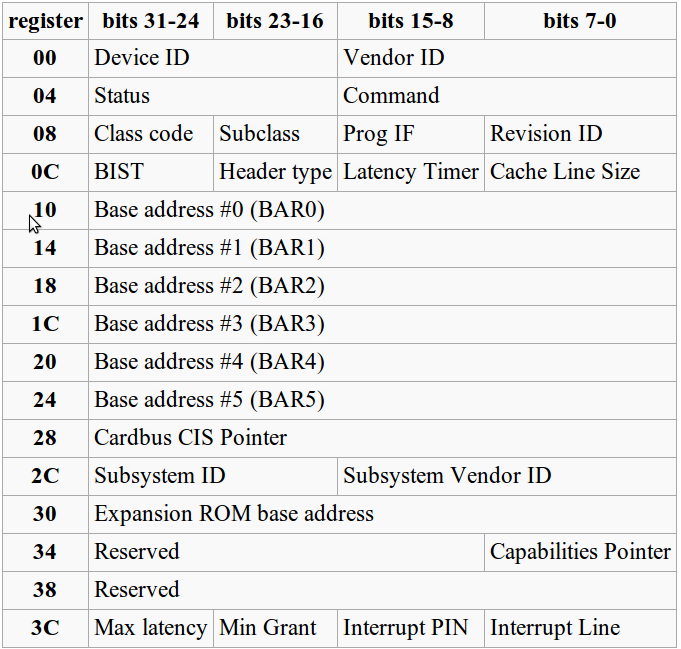
\includegraphics[scale=0.40]{/home/zhangchi/lab/report/pcicr.png}
\end{figure}

\item[PCI设备启动过程]:\\


在系统引导阶段,PCI硬件设备保持未激活状态,每个设备都没有被分配内存空间和I/O端口。但每个PCI主板均配备有能够处理PCI的固件(比如BIOS),固件通过读写PCI控制器中的寄存器,提供了对设备配置地址空间的访问。系统启动以后,固件通过扫描每个PCI设备,通过读取他们的配置地址空间,为每个设备分配相应的内存和I/O端口,为后面硬件驱动程序做好准备。


\item[如何使用PCI设备]:\\

当我们想查询一个特定PCI设备的配置地址空间时,我们需要向I/O地址$[\mathrm{0cf8}, \mathrm{0cfb}]$ 写入一个 4 bytes查询码指定总线号:设备号:功能号以及其配置地址空间中的查询位置。那么PCI Host Bridge将监听对于这个I/O端口的写入并在接受到写入数据后将相应的查询结果写入到 $[\mathrm{0cfc}, \mathrm{0cff}]$ , 我们从这个地址读出一个32位整数表示查询到的相应信息。

查询配置地址空间时,我们一般会从其6个BARS中得到特定设备的控制端口和数据端口信息,那么只要在初始化时将这些端口地址保存下来,就可以在PCI硬件驱动程序中通过向这些端口输入输出数据来达到控制PCI设备的目的了

\end{description}

更多更详细的内容可以参考网站:\burl{http://xwindow.angelfire.com/page13_1.html},上面介绍的内容已经足够我们理解JOS中的相应代码了。

\vspace{2em}
\hrule
\vspace{2em}

接下来我们看JOS中是如何对PCI设备进行编程的,这部分模块主要定义在kern/pci.c中,JOS在系统初始化时调用其中的 \funcname{pci\_init()} 进行设备初始化,首先来看一些最基本的东西:

\begin{lstlisting}[style=ccode, firstnumber=36, title={\scriptsize \ttfamily \bfseries kern/pci.c}]
static void
pci_conf1_set_addr(uint32_t bus,
		   uint32_t dev,
		   uint32_t func,
		   uint32_t offset)
{
	assert(bus < 256);
	assert(dev < 32);
	assert(func < 8);
	assert(offset < 256);
	assert((offset & 0x3) == 0);
	
	uint32_t v = (1 << 31) |		// config-space
		(bus << 16) | (dev << 11) | (func << 8) | (offset);
	outl(pci_conf1_addr_ioport, v);
}

static uint32_t
pci_conf_read(struct pci_func *f, uint32_t off)
{
	pci_conf1_set_addr(f->bus->busno, f->dev, f->func, off);
	return inl(pci_conf1_data_ioport);
}

static void
pci_conf_write(struct pci_func *f, uintint
e100_sw_reset(struct dev_e100 *e100) {
        outl(e100->reg_base[E100_IO] + CSR_PORT, PORT_SW_RESET);
        
        // delay about 10us
        int i = 0;
        for (i = 0; i < 8; i++) {
                inb (0x84);
        }

        e100_init(e100);

        return 1;
}
32_t off, uint32_t v)
{
	pci_conf1_set_addr(f->bus->busno, f->dev, f->func, off);
	outl(pci_conf1_data_ioport, v);
}
\end{lstlisting}


这三个函数是对PCI设备最基本的读状态和写状态的函数,其中 \funcname{ pci\_conf1\_set\_addr() } 负责设置需要读写的具体设备。这里涉及到的两个I/O端口定义在了文件最上方:


\begin{lstlisting}[style=ccode, firstnumber=12, title={\scriptsize \ttfamily \bfseries kern/pci.c}]
// PCI "configuration mechanism one"
static uint32_t pci_conf1_addr_ioport = 0x0cf8;
static uint32_t pci_conf1_data_ioport = 0x0cfc;
\end{lstlisting}

正是我们前面提到的两个端口。接下来我们看看它是怎么初始化PCI设备的,看到 \funcname{pic\_init()}:


\begin{lstlisting}[style=ccode, firstnumber=36, title={\scriptsize \ttfamily \bfseries kern/pci.c}]
static int 
pci_scan_bus(struct pci_bus *bus)
{
    int totaldev = 0;
    struct pci_func df;
    memset(&df, 0, sizeof(df));
    df.bus = bus;
	
    for (df.dev = 0; df.dev < 32; df.dev++) {
        uint32_t bhlc = pci_conf_read(&df, PCI_BHLC_REG);
        if (PCI_HDRTYPE_TYPE(bhlc) > 1)	    // Unsupported or no device
            continue;
		
        totaldev++;
		
        struct pci_func f = df;
        for (f.func = 0; f.func < (PCI_HDRTYPE_MULTIFN(bhlc) ? 8 : 1); f.func++) {
            struct pci_func af = f;
			
            af.dev_id = pci_conf_read(&f, PCI_ID_REG);
            if (PCI_VENDOR(af.dev_id) == 0xffff)
                continue;
			
            uint32_t intr = pci_conf_read(&af, PCI_INTERRUPT_REG);
            af.irq_line = PCI_INTERRUPT_LINE(intr);
			
            af.dev_class = pci_conf_read(&af, PCI_CLASS_REG);
            if (pci_show_devs)
                pci_print_func(&af);
            pci_attach(&af);
        }
    }
	
    return totaldev;
}

int
pci_init(void)
{
	static struct pci_bus root_bus;
	memset(&root_bus, 0, sizeof(root_bus));
	
	return pci_scan_bus(&root_bus);
}
\end{lstlisting}

\begin{enumerate}
\item{\funcname{pci\_init()}中,root\_bus被全部清0,然后交给\funcname{pci\_scan\_bus()}扫描这条总线上的所有设备,说明在JOS中E100是被放置在0号总线上的}
\item{\funcname{pci\_scan\_bus()} 中顺次查找0号总线上的32个设备,如果发现其存在,那么顺次扫描它们每个功能对应的配置地址空间,将一些关键的控制参数读入pci\_func进行保存,其中pci\_func的结构如下:

\begin{lstlisting}[style=ccode, firstnumber=11, title={\scriptsize \ttfamily \bfseries kern/pci.h}]
struct pci_func {
    struct pci_bus *bus;	// Primary bus for bridges

    uint32_t dev;
    uint32_t func;

    uint32_t dev_id;
    uint32_t dev_class;

    uint32_t reg_base[6];
    uint32_t reg_size[6];
    uint8_t irq_line;
};
\end{lstlisting}

对于网卡驱动来说,最重要的就是其reg\_base数组,这是我们用于向E100发送命令的地址端口,在后面的初始化程序中我们需要将其记录下来。

}

\item{得到pci\_func之后,它被传入\funcname{pci\_attach()}去查找是否为已存在的硬件,如果匹配成功,则使用预设好的程序初始化该硬件

\begin{lstlisting}[style=ccode, firstnumber=67, title={\scriptsize \ttfamily \bfseries kern/pci.c}]
static int __attribute__((warn_unused_result))
pci_attach_match(uint32_t key1, uint32_t key2,
		 struct pci_driver *list, struct pci_func *pcif)
{
    uint32_t i;
	
    for (i = 0; list[i].attachfn; i++) {
        if (list[i].key1 == key1 && list[i].key2 == key2) {
            int r = list[i].attachfn(pcif);
            if (r > 0)
                return r;
            if (r < 0)
                cprintf("pci_attach_match: attaching "
                    "%x.%x (%p): e\n",
                    key1, key2, list[i].attachfn, r);
        }
    }
    return 0;
}

static int
pci_attach(struct pci_func *f)
{
    return
        pci_attach_match(PCI_CLASS(f->dev_class), 
                PCI_SUBCLASS(f->dev_class),
                &pci_attach_class[0], f) ||
        pci_attach_match(PCI_VENDOR(f->dev_id), 
                PCI_PRODUCT(f->dev_id),
                &pci_attach_vendor[0], f);
}
\end{lstlisting}


}
\end{enumerate}

到这里PCI设备的初始化就结束了,接下来我们要尝试写一个E100网卡的初始化过程。

\begin{lstlisting}[style=exercise]
|Exercise 3|. Implement an attach function to initialize the 82559ER. Add an entry to the pci_attach_vendor array in kern/pci.c to trigger your function if a matching PCI device is found. The vendor ID and device ID for the 82559ER can be found in Section 4 of the developer manual. You should also see these listed when JOS scans the PCI bus while booting.

After enabling the E100 device via pci_func_enable, your attach function should record the IRQ line and base I/O port assigned to the device so you'll be able to communicate with the E100.

We have provided the kern/e100.c and kern/e100.h files for you so that you do not need to mess with the make system. You may still need to include the e100.h file in other places in the kernel.

When you boot your kernel, you should see it print that the PCI function of the E100 card was enabled. Your code should now pass the pci attach test of make grade.
\end{lstlisting}

第一步我们查阅手册得到E100的Vender ID为8086h,Device ID为1229h,然后将初始化程序作为驱动程序的一部分定义在kern/e100.c中,先撰写头文件kern/e100.h:

\begin{lstlisting}[style=ccode, title={\scriptsize \ttfamily \bfseries kern/e100.h}]
#ifndef JOS_KERN_E100_H
#define JOS_KERN_E100_H

#include <kern/pci.h>

#define E100_VENDOR		0x8086
#define E100_DEVICE		0x1209

int e100_attach(struct pci_func *pcif);

#endif	// JOS_KERN_E100_H
\end{lstlisting}

然后是主过程,定义了一个e100记录其相应的设备信息:

\begin{lstlisting}[style=ccode, title={\scriptsize \ttfamily \bfseries kern/e100.c}]
// LAB 6: Your driver code here

#include <inc/x86.h>
#include <inc/stdio.h>

#include <kern/e100.h>

struct pci_func e100;

int 
e100_attach(struct pci_func *pcif) 
{
    pci_func_enable(pcif);
    e100.bus = pcif->bus;
    e100.dev_id = pcif->dev_id;
    e100.dev_class = pcif->dev_class;
    int i;
    for (i = 0; i < 6; i++) {
    	e100.reg_base[i] = pcif->reg_base[i];
        e100.reg_size[i] = pcif->reg_size[i];
        cprintf ("zhangchi: The %dth Bar: base = %x, size = %x\n", 
            i, e100.reg_base[i], e100.reg_size[i]);
    }
    e100.irq_line = pcif->irq_line;

    return 0;
}
\end{lstlisting}

接下来修改kern/pci.c中的pci\_attach\_vendor数组,把我们的E100初始化程序添加进去:

\begin{lstlisting}[style=ccode, firstnumber=31, title={\scriptsize \ttfamily \bfseries kern/pci.c}]
// pci_attach_vendor matches the vendor ID and device ID of a PCI device
struct pci_driver pci_attach_vendor[] = {
	{ E100_VENDOR, E100_DEVICE, &e100_attach }, 
	{ 0, 0, 0 },
};
\end{lstlisting}

然后make qemu启动JOS,应该能看到E100网卡被顺利激活了:

\begin{lstlisting}[style=console]
enabled interrupts: 1 2
	     Setup timer interrupts via 8259A
enabled interrupts: 0 1 2
	     unmasked timer interrupt
PCI: 00:00.0: 8086:1237: class: 6.0 (Bridge device) irq: 0
PCI: 00:01.0: 8086:7000: class: 6.1 (Bridge device) irq: 0
PCI: 00:01.1: 8086:7010: class: 1.1 (Storage controller) irq: 0
PCI: 00:01.3: 8086:7113: class: 6.80 (Bridge device) irq: 9
PCI: 00:02.0: 1013:00b8: class: 3.0 (Display controller) irq: 0
PCI: 00:03.0: 8086:1209: class: 2.0 (Network controller) irq: 11
PCI function 00:03.0 (8086:1209) enabled
zhangchi: The 0th Bar: base = f2020000, size = 1000
zhangchi: The 1th Bar: base = c040, size = 40
zhangchi: The 2th Bar: base = f2040000, size = 20000
zhangchi: The 3th Bar: base = 0, size = 0
zhangchi: The 4th Bar: base = 0, size = 0
zhangchi: The 5th Bar: base = 0, size = 0
FS is running
FS can do I/O
\end{lstlisting}

可以看到第二个端口应该就是我们以后进行操作的I/O端口c040,空间大小为40h = 64 bytes


\subsubsection{E100 Reset}


\begin{lstlisting}[style=exercise]
|Exercise 4|. Add code to your attach function to reset the 82559ER. If you set the -debug-e100 flag, QEMU should tell you if the reset was successfully. It will print something like this after JOS starts scanning the PCI bus:

EE100   nic_reset               0xacea498

There will also be a few nic_reset's before JOS starts; those are the BIOS itself resetting the device.
\end{lstlisting}


这一段的MIT提供的资料是相对来说比较详尽的,还记得我们前面打印出来的c040地址么?这个地方就是我们要写入CSR的端口。CSR(Control/Status Registers)是我们对于E100网卡的控制字,如前面所说,它是一个64 bytes的地址空间,其中我们最需要关注的是它的前12个bytes,称为SCB(System Control Block),我们对网卡的主要控制主要是对于SCB相应参数的进行设置。其布局如下:

\begin{figure}[htp]
\centering
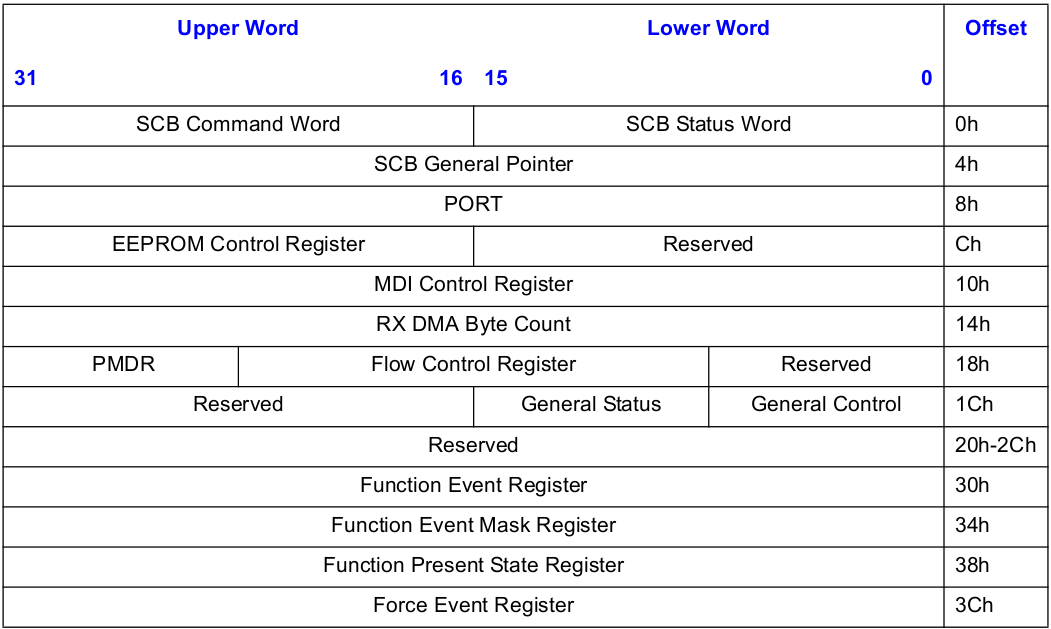
\includegraphics[scale=0.30]{/home/zhangchi/lab/report/csr.png}
\end{figure}

对于重设网卡,是采用的PORT Interface的形式进行控制,详见Manual的6.3.3 PORT Interface。这里E100允许我们只对SCB中的PORT设置特定值以后就执行相应的功能,比如说有:


\begin{figure}[htp]
\centering
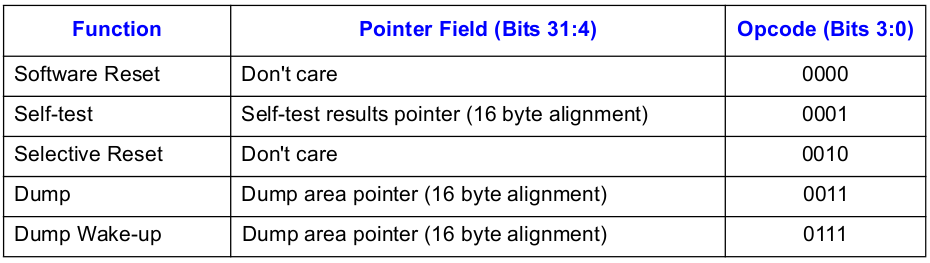
\includegraphics[scale=0.30]{/home/zhangchi/lab/report/reset.png}
\end{figure}

从这个表格看出,我们只需要对PORT字段写入全0就可以达到重启的目的了。

但是在进行编码之前,我们需要对头文件进行一些修改,方便后续的程序编写。

\begin{lstlisting}[style=ccode, title={\scriptsize \ttfamily \bfseries kern/e1000.h}]
#ifndef JOS_KERN_E100_H
#define JOS_KERN_E100_H

#include <kern/pci.h>

#define E100_VENDOR		0x8086
#define E100_DEVICE		0x1209

#define E100_MEMORY     0
#define E100_IO         1
#define E100_FLASH      2

#define CSR_SCB         0x0
#define CSR_STATUS      0x0
#define CSR_US          0x0
#define CSR_STATACK     0x1
#define CSR_COMMAND     0x2
#define CSR_UC          0x2
#define CSR_INT         0x3
#define CSR_GP          0x4
#define CSR_PORT        0x8


#define PORT_SW_RESET   0x0
#define PORT_SELF_TEST  0x1
#define PORT_SEL_RESET  0x2

int e100_attach(struct pci_func *pcif);

#endif	// JOS_KERN_E100_H
\end{lstlisting}


\begin{enumerate}
\item{在手册中的4.1 PCI Configuration Space,对于E100而言,PCI配置中提供的6个地址中的前三个分别为

\begin{enumerate}
\item{CSR Memory Mapped Base Address Register}
\item{CSR I/O Mapped Base Address Register}
\item{Flash Memory Mapped Base Address Register}
\end{enumerate}

因为我们只使用I/O端口对CSR进行控制,不使用内存地址的原因资料中也提到了,有可能因为编译器的原因使得地址端口失效,所以最稳固的方法还是使用I/O的方式。这三个地址在初始化时已经被载入到e100.reg\_base[0-2]中了。在使用他们的基址的时候,我们为他们定义了相应的数组索引位置
}
\item{定义了一系列SCB字段在CSR中的位移,以便于后面我们使用in和out指令对他们进行读写操作}
\item{预定义了三条PORT Interface指令}
\end{enumerate}

作这项工作中我大量参考了\burl{http://code.google.com/p/os-xv6-network/source/browse/trunk/dev/e100.h}提供的参数,节省了我大量的时间,对作者表示感谢。


然后就可以真正开始对网卡进行重启了:


\begin{lstlisting}[style=ccode, title={\scriptsize \ttfamily \bfseries kern/e100.c}]
// LAB 6: Your driver code here

#include <inc/x86.h>
#include <inc/stdio.h>

#include <kern/e100.h>

struct pci_func e100;

static void e100_sw_reset(struct pci_func e100);

int 
e100_attach(struct pci_func *pcif) 
{
    pci_func_enable(pcif);
    e100.bus = pcif->bus;
    e100.dev_id = pcif->dev_id;
    e100.dev_class = pcif->dev_class;
    int i;
    for (i = 0; i < 6; i++) {
    	e100.reg_base[i] = pcif->reg_base[i];
        e100.reg_size[i] = pcif->reg_size[i];
    }
    e100.irq_line = pcif->irq_line;

    e100_sw_reset(e100);
}

static void
e100_sw_reset(struct pci_func e100) {
    outl(e100.reg_base[E100_IO] + CSR_PORT, PORT_SW_RESET);

    // delay about 10us
    int i = 0;
    for (i = 0; i < 8; i++) {
        inb (0x84);
    }
}

\end{lstlisting}

注意不要忘了按照MIT材料的提示重启后delay 一段时间再返回。使用make qemu QEMUEXTRA="-debug-e100"启动JOS应该可以看到网卡的重启消息:

\begin{lstlisting}[style=console]
EE100	nic_init                
EE100	pci_reset               0x9566008
EE100	nic_init                macaddr:  52 54 00 12 34 56
EE100	nic_reset               0x9566008
EE100	nic_selective_reset     checksum=0xbe34
EE100	nic_init                model=i82559er,macaddr=52:54:00:12:34:56
EE100	nic_reset               0x9566008
EE100	nic_selective_reset     checksum=0xbe34
EE100	pci_mmio_map            region 0, addr=0xf2020000, size=0x00001000, type=8
EE100	pci_map                 region 1, addr=0x0000c040, size=0x00000040, type=1
EE100	pci_mmio_map            region 2, addr=0xf2040000, size=0x00020000, type=0
6828 decimal is 15254 octal!
Hooray! Passed all test cases for stdlib!!
Physical memory: 66556K available, base = 640K, extended = 65532K
check_page_alloc() succeeded!
page_check() succeeded!
check_boot_pgdir() succeeded!
enabled interrupts: 1 2
	     Setup timer interrupts via 8259A
enabled interrupts: 0 1 2
	     unmasked timer interrupt
PCI: 00:00.0: 8086:1237: class: 6.0 (Bridge device) irq: 0
PCI: 00:01.0: 8086:7000: class: 6.1 (Bridge device) irq: 0
PCI: 00:01.1: 8086:7010: class: 1.1 (Storage controller) irq: 0
PCI: 00:01.3: 8086:7113: class: 6.80 (Bridge device) irq: 9
PCI: 00:02.0: 1013:00b8: class: 3.0 (Display controller) irq: 0
PCI: 00:03.0: 8086:1209: class: 2.0 (Network controller) irq: 11
EE100	pci_mmio_map            region 0, addr=0xf2020000, size=0x00001000, type=8
EE100	pci_map                 region 1, addr=0x0000c040, size=0x00000040, type=1
EE100	pci_mmio_map            region 2, addr=0xf2040000, size=0x00020000, type=0
PCI function 00:03.0 (8086:1209) enabled
EE100	eepro100_write4         addr=Port+0 val=0x00000000
EE100	nic_reset               0x9566008
EE100	nic_selective_reset     checksum=0xbe34
FS is running
\end{lstlisting}




\subsubsection{E100 Structure}

其实这里Intel的手册挺让人费解的,我读了以后发现CU其实就是负责发送数据的模块,RU就是接收数据的模块,按道理两个是相对的,那么CU应该称为Transmit Unit才对,Intel却命名为Control Unit,让人感觉这两个模块是分立的,并且CU有控制RU一样。

对于CU和RU的讨论我们要等到将DMA Ring看完以后才能完整的描述,我们先来看DMA Rings

\subsubsection{DMA Rings}

根据资料的描述,DMA Rings就是系统为E100在内存中开辟的一片区域,用于网卡使用DMA缓存当前的收发数据的。一个DMA Rings在申请好以后,就可以将其所在的物理地址通知给E100的DMA控制器,那么E100就可以在不占用CPU的情况下自己根据内存中的数据开始进行收发操作了。\highlight{实际情况中内存里应该有两条DMA Rings},一个专门用于放置待发送的数据(Control Block list, CBL),一个专门放置接受到的数据(Receive Frame Area, RFA)。

因为采取了这样的操作模式,所以提示我们E100是根据DMA Rings中的内容进行工作的。接下来我们就会详细讲述利用CU发送数据时数据包格式是如何用Control Block(CB)进行描述的。E100读取CB中的设置,然后进行相应的发送操作,当工作完成后,\highlight{通过引发中断或者改变DMA Rings相应的状态位来提示系统工作已完成}。我们可以修改CB中相应场位的设置,来改变E100的工作模式。

上面是E100自动进行工作的一种方式,如果我们需要人为的干预E100的运行的话,\highlight{还可以向CSR中的SCB寄存器写入相应的控制指令},比如终止运行等,来改变其运行状态。

所以,在完成这个部分的工作前,我们需要了解两方面重要的内容:

\begin{enumerate}
\item{CB (Control Block)的控制设置}
\item{SCB (System Control Block)的控制设置}
\end{enumerate}

在了解 DMA Rings 的相关结构以后,我们会结合DMA Rings来进一步阐述这些控制设置在 DMA Rings上运行的效果。

\subsection{Device Driver Organization}


\subsection{Transmitting Packets}

前面提到DMA Rings主要分为两种用途:发送和接受。
\begin{itemize}

\item{发送数据的DMA Rings是由若干个CB (Control Block)组成的,这些CB通过指针连接成一个环状的结构CBL(Control Block List)。}
\item{接受数据的DMA Rings由若干个RFD (Receive Frame Descriptior)组成,也是连成环状,称为RFA (Receive Frame Area)}
\end{itemize}

这个阶段我们主要关注发送,发送是由CU模块来完成的。

\highlight{CB是一个通用的概念},即使是只在发送时用到,但是因为CU执行的不止一种命令,所以根据不同命令的需要对CB进行更加细致的规定。只有CB的前三个成员Control, Status和Link在各个应用场景中都是相同的,接下来的Command Specific Data才是根据不同的命令发生变化的。一个CB的结构在Intel的开源手册中的6.4.1.1 General Action Command Format中可以找到具体格式,如下图所示:


\begin{figure}[htp]
\centering
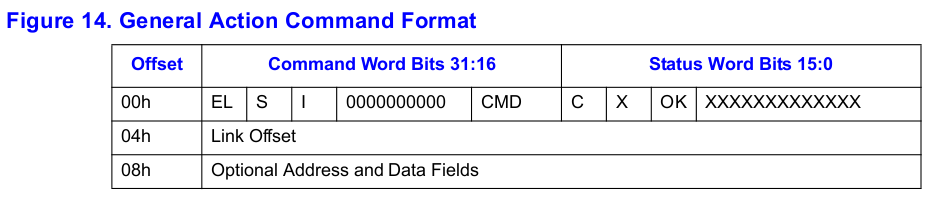
\includegraphics[scale=0.30]{/home/zhangchi/lab/report/cbaction.png}
\end{figure}

其中有三个位置是特别值得我们关注的:

\begin{itemize}
\item{S:如果该位被设置为1,那么当E100的\highlight{CU}执行完此CB的命令之后,将停止运行进入挂起状态(Suspend),只有使用SCB对E100下达恢复运行(Resume)指令后,CU模块才会重新运行,重新运行开始时执行的地址是该CB的Link Address指向的下一CB。注意,这里要注意\highlight{发送和接受是互相独立不干扰的},所以CU停止工作的时候有可能RU还在正常运行,注意明确他们两个结构的概念。}
\item{Status Word Bits中的C位:在操作CU执行任意CB上的命令时,\highlight{程序员首先应该负责手动清除该位上的值},将其置为0。那么当CU模块执行完任务后,这个位置被设置成1。就可以检测某些指令的执行情况了。比如发送数据时由于数据包比较大,从CU获取到CB开始执行到发送完毕需要耗费一定的时间,
}
\item{CMD:CB支持的不同的操作类型,具体操作类型可以在手册的6.4.2 Specific Action Commands中找到,大致有以下几种操作:

\begin{itemize}
\item{NOP (000b)}
\item{Individual Address Setup (001b)}
\item{Configure (010b)}
\item{Multicast Setup (011b)}
\item{Transmit (100b)}
\item{Load Microcode (101b)}
\item{Dump (110b)}
\item{Diagnose (111b)}
\end{itemize}

在这次实验中我们在CU模块的操作只会遇到两个:NOP和Transmit,严格的说只要使用Transmit就好了,但是在写的时候我们可以用NOP来进行一些测试,来检测程序的正确性。NOP的作用就是使CU在处理到该CB时什么事情也不作,\highlight{但是相应的状态位S、C等等都会对CU的执行有作用}。所以我们可以利用NOP指令设置S位\highlight{使其停止在某个CB上},然后利用debug的输出信息进行调试,而不用去理会Transimit指令中其他那些乱七八糟的参数的设置。
}
\end{itemize}

看完CB的相关字段说明,我们可以将这些状态定义到头文件里方便后续的设置和读取判断了:

\begin{lstlisting}[style=ccode, title={\scriptsize \ttfamily \bfseries kern/e100.h}]
// Control Block Command
#define CBF_EL          0x8000
#define CBF_S           0x4000
#define CBF_I           0x2000

#define CBC_NOP         0x0
#define CBC_IAS         0x1
#define CBC_CONFIG      0x2
#define CBC_MAS         0x3
#define CBC_TRANSMIT    0x4
#define CBC_LOADMC      0x5
#define CBC_DUMP        0x6
#define CBC_DIAGNOSE    0x7

// Control Block Status
#define CBS_F           0x0800
#define CBS_OK          0x2000
#define CBS_C           0x8000
\end{lstlisting}

\subsubsection{C Structures}


上面描述的是CB的一些通用概念,具体到发送包指令Transmit的时候,我们将这样一连串的CB称为TCBs (Transmit Command Blocks)。在MIT资料中已经有一个形象的图为我们展示出了TCB的串联结构,更详细的信息可以在手册中的6.4.2.5 Transmit找到。这个是TCB的一个布局图。

\begin{figure}[htp]
\centering
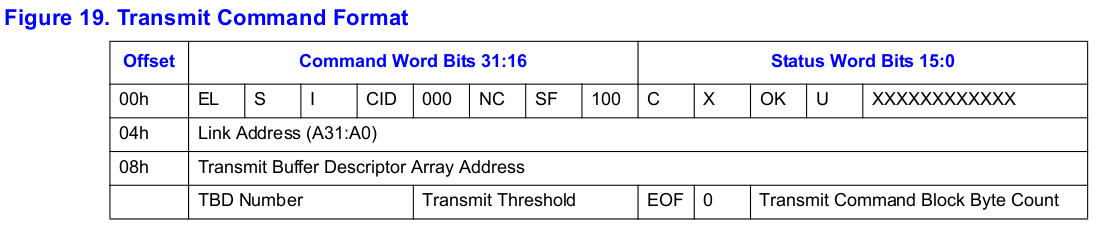
\includegraphics[scale=0.30]{/home/zhangchi/lab/report/tcb.png}
\end{figure}

可以看到,虽然TCB的结构比CB更细化了,但是我们现在还不需要关注它的设置的细节,第一步我们先考虑\highlight{在内存中分配空间和建立起相应的TCB结构}。这就需要结合CU的工作方式来阐述它是如何读取和使用TCB的了。以下列出了使用TCBs发送数据包的全过程:

\begin{enumerate}
\item{首先在内存中建立起TCBs的环状结构}
\item{将其中第一个TCB的物理地址写入CU的General Pointer,通知其要操作的TCB所在的内存位置}
\item{给CU一个Start指令,CU开始工作}
\item{如果环状的TCB中所有的S位都是0,那么CU将根据Link Address无限循环的处理这些TCB,每次执行完成以后,以中断和修改TCB中C状态位来表明任务已完成(后面我们会说明处理这些消息的方式,现在先不用管)}
\item{如果CU碰到了某个TCB的S被设置为1,那么处理完该TCB之后,CU进入Suspend状态,等待用户发送Resume命令恢复运行,那么CU将从当前TCB的下个TCB开始执行}
\end{enumerate}


这只是硬件的执行机制,我们现在要考虑在TCBs上实现一个\highlight{支持多数据包发送的排队系统},应该注意些什么?

\begin{enumerate}
\item{首先要记录当前TCB中哪些块是等待被发送的,哪些是可以被重新利用的}
\item{其次要做好相应S位设置,让CU在发送完需要发送的包之后就停下来}
\end{enumerate}

考虑到上述两点,我们设计出的系统是这样描述TCB的:

\begin{lstlisting}[style=ccode, title={\scriptsize \ttfamily \bfseries kern/e100.h}]
#define TCB_MAXSIZE     1518
#define CB_MAX_NUM      10

// Transmit Command Blocks
struct tcb {
    uint32_t tcb_tbd_array_addr;
    uint16_t tcb_byte_count;
    uint8_t tcb_thrs;
    uint8_t tcb_tbd_count;
    char tcb_data[TCB_MAXSIZE];
};

// Control Blocks
struct cb {
    volatile uint16_t cb_status;
    uint16_t cb_control;
    uint32_t cb_link;

    union cb_cmd_spec_data {
        struct tcb tcb;
    } cb_cmd_spec;

    struct cb *prev, *next;
    physaddr_t phy_addr;   
};

// Control Block List
struct cbl {
    int cb_avail;
    int cb_wait;

    struct cb *start;
    struct cb *front, *rear;
};
\end{lstlisting}

解释一下这些结构:

\begin{itemize}
\item{tcb:直接按照MIT给出的结构定义的,没什么好说}
\item{cb: 这里有两点值得注意:
\begin{enumerate}
\item{union结构cb\_cmd\_spec是根据不同指令的需要说明的,其实这里我们只用到了Transmit指令,所以union中只有一个成员看着比较别扭,但是这样写更具有\highlight{扩展性和维护性},当需要使用到其他指令时,直接在cb\_cmd\_spec里添加其他的数据结构即可}
\item{在cb\_cmd\_spec的后面我们增加了三个成员prev, next和phy\_addr,这个和手册上关于CB的定义是不符的,但是并不影响CU的执行,主要是为了我们自己在后续操作中的方便,}
\end{enumerate}
}
\item{cbl: 这里维护了几个值,分别说明一下:
\begin{itemize}
\item{cb\_avail: 表示当前有多少个闲置的TCB可以用来放置数据以发送}
\item{cb\_wait: 表示当前有多少个TCB正在处于等待发送状态}
\item{很明显上面两者相加应该等于所有TCB的总数,在这里应该是我们定义的CB\_MAX\_NUM = 10}
\item{start: 所有TCB中的第一个TCB,用于开始的时候初始化CU用}
\item{front和rear: 表示当前正在等待发送的TCB的起始和结尾}

\end{itemize}
}
\end{itemize}

那么这个系统是如何根据cbl中定义的结构工作的呢?

\begin{enumerate}
\item{初始的时候front = start, rear = start$\rightarrow$prev,表示当前等待发送的数据包为空,并且cb\_avail = CB\_MAX\_NUM, cb\_wait = 0}
\item{当需要发送一个数据包时,将其添加到rear后面,并且移动rear指针,同时增加cb\_wait, 减少cb\_avail}
\item{当确认等待数据包发送时,检查front指向TCB的C状态是否为1,可以的话则将front向后移动,表示front指向的数据包已经被CU发送。同时减少cb\_wait, 增加cb\_avail}

\end{enumerate}

那么相应的边界状态比如队列空或者队列满就可以很容易的通过 cb\_wait 和 cb\_avail 检测出来了。我们在这里还没有结合控制位中S的设置来说明CU的工作方式,这个在讲发送数据包的时候会讲到移动指针时会如何进行Suspend位的设置,具体请参考\ref{cususpend}

\vspace{2em}
\hrule
\vspace{2em}

好了到这里我们已经清楚了一个TCB结构是如何被建立起来并且在后续过程中维护的详细过程,现在我们可以考虑建立起这样的结构了:

\begin{lstlisting}[style=exercise]
|Exercise 5|. Construct a control DMA ring for the CU to use. You do not need to worry about configuring the device because the default setting are fine. You also do not need to worry about setting up the device MAC address because the emulated E100 has one already configured.
\end{lstlisting}

首先为了程序的易于管理,我们新定义了一个结构nic:

\begin{lstlisting}[style=ccode, title={\scriptsize \ttfamily \bfseries kern/e100.h}]
// Network Interface Card
struct nic {
    uint32_t io_base;
    uint32_t io_size;

    struct cbl cbl;
};\end{lstlisting}

nic是用于编写E100网卡驱动中所有过程中一个记录需要使用到的资源的工具,管理我们用到的I/O端口和CBL、RFA等等。

注意在前面的初始化硬件过程中添加上nic的初始化过程:

\begin{lstlisting}[style=ccode, title={\scriptsize \ttfamily \bfseries kern/e100.c}]
struct nic nic;

int
e100_attach(struct pci_func *pcif) 
{
    pci_func_enable(pcif);
    e100.bus = pcif->bus;
    e100.dev_id = pcif->dev_id;
    e100.dev_class = pcif->dev_class;
    int i;
    for (i = 0; i < 6; i++) {
    	e100.reg_base[i] = pcif->reg_base[i];
        e100.reg_size[i] = pcif->reg_size[i];
    }
    e100.irq_line = pcif->irq_line;

    // Initialize NIC
    nic.io_base = pcif->reg_base[E100_IO];
    nic.io_size = pcif->reg_size[E100_IO];

    e100_init ();

    return 0;
}
\end{lstlisting}

在初始化的第一步我们先需要为TCB分配\highlight{物理空间},为什么要强调是物理地址呢?

因为一开始我犯了一个错误,我特别在系统\highlight{虚拟地址空间}里在KERNBASE以上找了一块连续的区域(我找的是KERNBASE + PGSIZE开始),专门映射这些TCB。但是后来就发现这样映射是完全没有必要的:

\begin{itemize}
\item{首先如果将其映射到虚拟地址上是为了方便内核里使用指针访问这些TCB的话,那么我们利用\funcname{page\_alloc()} 得到这些物理页面对应的 struct Page 的时候,就可以利用page2kva (Page)的虚拟地址访问他们了}

\item{其次,前面我们使用page2kva (Page)访问的前提,是因为在内存管理的Lab中,KERNBASE以上的空间全部被\highlight{静态映射}成一一对应的物理内存(注意回顾静态映射的概念,就是被映射到的物理页\highlight{没有改变其引用数},方便我们可以重用这些物理页,静态映射的意义就只是单纯提供一个顺序访问所有物理地址的转换而已)}

\item{如果我们设置一个KERNBASE上的区域专门映射我们分配到的TCB物理页面,那么该虚拟地址原来对应的真实物理页就要被卸载,如果在未来的某个时候这个真实物理页被分配后需要用page2kva这样的地址进行访问,那么映射就会失败,其访问到的是我们现在安装上的TCB的物理页,这样就会造成系统的崩溃}
\end{itemize}

{\bfseries \large \color{red} 所以为TCB的物理页分配虚拟地址空间不仅是没必要的,在有的时候更可能造成系统的崩溃。感谢张顺廷湿胸指出了我理解上的错误!}

\vspace{2em}

真实分配的时候,我们为CB\_MAX\_NUM个TCB每个分配一个物理页(实际上一个TCB大概只占用半页的样子,因为tcb\_data最大才1518个bytes而已,但是这样比较方便操作),于是初始化的程序如下:

\label{cblalloc}

\begin{lstlisting}[style=ccode, title={\scriptsize \ttfamily \bfseries kern/e100.c: cbl\_alloc()}]
/**
 * Allocate CB_MAX_NUM pages, each page for a control block
 */
static void
cbl_alloc () {
    int i, r;
    struct Page *p;
    struct cb *prevcb = NULL;
    struct cb *currcb = NULL;

    // Allocate physical page for Control block
    for (i = 0; i < CB_MAX_NUM; i++) {

        if ((r = page_alloc (&p)) != 0)
            panic ("cbl_init: run out of physical memory! %e\n", r);

        p -> pp_ref ++;
        memset (page2kva (p), 0, PGSIZE);

        currcb = (struct cb *)page2kva (p);
        currcb->phy_addr = page2pa (p);


        if (i == 0)
            nic.cbl.start = currcb;
        else {
            prevcb->cb_link = currcb->phy_addr;
            prevcb->next = currcb;
            currcb->prev = prevcb;
        }

        prevcb = currcb;
    }

    prevcb->cb_link = nic.cbl.start->phy_addr;
    nic.cbl.start->prev = prevcb;
    prevcb->next = nic.cbl.start;

    nic.cbl.cb_avail = CB_MAX_NUM;
    nic.cbl.cb_wait = 0;

    nic.cbl.front = nic.cbl.start;
    nic.cbl.rear = nic.cbl.start->prev;
}
\end{lstlisting}

通过\funcname{page\_alloc()} 拿到物理页之后,第一记得增加它的ref数,第二记得清空所有的数据。

\vspace{2em}
\hrule
\vspace{2em}

TCB结构建立完毕以后,我们可以考虑使用CU在TCB上跑一跑了。从这里开始就涉及到对于CU的操作字的问题。首先回顾一下我们在建立TCB以后可能需要进行的操作:

\begin{enumerate}
\item{将其中第一个TCB的物理地址写入CU的General Pointer,通知其要操作的TCB所在的内存位置}
\item{给CU一个Start指令,CU开始工作}
\item{如果环状的TCB中所有的S位都是0,那么CU将根据Link Address无限循环的处理这些TCB,每次执行完成以后,以中断和修改TCB中C状态位来表明任务已完成(后面我们会说明处理这些消息的方式,现在先不用管)}
\item{如果CU碰到了某个TCB的S被设置为1,那么处理完该TCB之后,CU进入Suspend状态,等待用户发送Resume命令恢复运行,那么CU将从当前TCB的下个TCB开始执行}
\end{enumerate}

在这里首先回答一下关于CU\highlight{执行完成后的响应问题}。如果让CU使用中断的方式提醒我们,效率会比较高,但是比较麻烦的是要去处理中断响应。而如果使用轮询的方式的话,根据我们CBL的结构,只需要每次测试front头的C状态位是否完成即可知道任务的完成状态,非常方便。

\label{scb}

我们带着这些需求来看看具体操作方法。控制CU是通过向SCB中写入相应的控制字决定的,具体规定在手册的6.3.2 System Control Block (SCB)中规定:

\begin{figure}[htp]
\centering
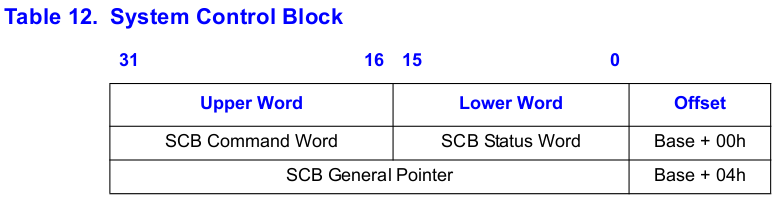
\includegraphics[scale=0.30]{/home/zhangchi/lab/report/scb.png}
\end{figure}

最主要的两个部分是控制字和状态字:

\begin{description}
\item[控制字]:\\
\begin{figure}[htp]
\centering
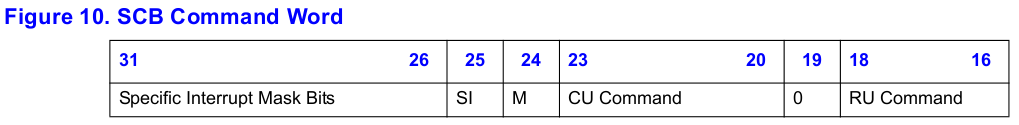
\includegraphics[scale=0.30]{/home/zhangchi/lab/report/scbcmd.png}
\end{figure}

我们主要需要关注三个字段:

\begin{itemize}
\item{M: 当控制字的这个位被设置成1,那么CU将不会发出任何中断,这个位正是当我们屏蔽中断时第一个需要给出的命令}
\item{CUC (CU Command): 这里对CU的控制命令有以下几种:

\begin{enumerate}
\item{0000 NOP}
\item{0001 CU Start}
\item{0010 CU Resume}
\item{0100 Load Dump Counters Address}
\item{0101 Dump Statistical Counters}
\item{0110 Load CU Base}
\item{0111 Dump and Reset Statistical Counters}
\item{1010 CU Static Resume} 
\end{enumerate}

我们要用到的主要是\highlight{CU Start}和\highlight{CU Resume},他们对应的需求为:

\begin{itemize}
\item{在建立好TCB并且给CU设置好TCB的地址以后,发出一个CU Start指令,CU开始工作}
\item{当CU在某个TCB因为S位被挂起以后,发出一个CU Resume指令可以让其恢复工作}
\end{itemize}

手册读到这里我们可以把相应的设置场位定义到kern/e100.h中了:

\begin{lstlisting}[style=ccode, title={\scriptsize \ttfamily \bfseries kern/e100.h}]
// CU Command Word
#define CUC_NOP         0x00
#define CUC_START       0x10
#define CUC_RESUME      0x20
#define CUC_LD_COUNTER  0x40
#define CUC_DUMP_SCNT   0x50
#define CUC_LOAD_BASE   0x60
#define CUC_DUMP_RSCNT  0x70
#define CUC_SRESUME     0xa0
\end{lstlisting}

}
\item{RUC (RU Command): 这个我们在后面\ref{scbru}会详细讲述}
\end{itemize}

看到这里,我们已经知道\highlight{如何关闭CU的中断}、使其\highlight{开始}和\highlight{恢复}执行,但是在开始前需要将TCB的地址告诉CU使其能够开始运行,这个如何设置?这里就涉及到SCB中General Pointer的设置了:

\begin{figure}[htp]
\centering
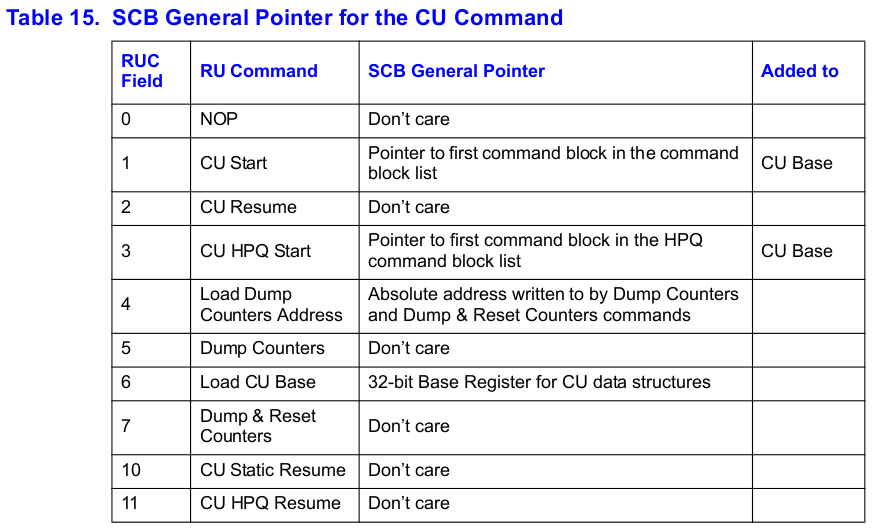
\includegraphics[scale=0.30]{/home/zhangchi/lab/report/scbgp.png}
\end{figure}

General Pointer是SCB中根据不同的命令设置的一个场位,\highlight{提供某些命令执行时需要的数据},比如这里我们只需要关注CU Start命令,在执行该命令前,General Pointer里必须写入开始执行的TCB的物理地址,那么CU Start时就可以从该TCB开始执行。而CU Resume就不需要,因为其下一次运行的TCB地址已经在被Suspend的时候被写入了内部寄存器。

设置General Pointer只需要像写入SCB的状态字和控制字一样直接像相应的I/O端口写入值即可。

\item[状态字]:\\
\begin{figure}[htp]
\centering
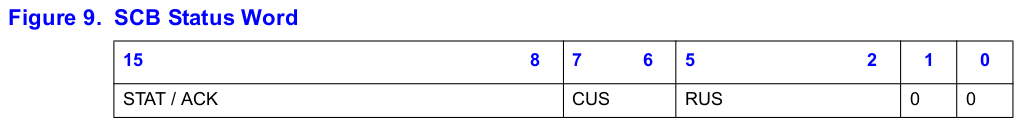
\includegraphics[scale=0.30]{/home/zhangchi/lab/report/scbstatus.png}
\end{figure}

这里我们只需要关注CU的状态字即可,它主要可能有以下状态:

\begin{enumerate}
\item{00: Idle}
\item{01: Suspend}
\item{10: LPQ Active}
\item{11: HQP Active}
\end{enumerate}

后面两个我都不知道是干吗的,这次实验里只需要知道前两个即可,因为如果不是前面两个的停止状态,那么当前CU肯定是在工作状态,然后将该状态值也定义到头文件里:


\begin{lstlisting}[style=ccode, title={\scriptsize \ttfamily \bfseries kern/e100.h}]
// CU Status Word
#define CUS_MASK        0xc0
#define CUS_IDLE        0x00
#define CUS_SUSPENDED   0x40
#define CUS_LPQ_ACTIVE  0x80
#define CUS_HQP_ACTIVE  0xc0
\end{lstlisting}

CUS\_MASK是由于要从SCB中读取其状态但CUS又是在中间的位置,所以先要用CUS\_MASK取出CUS相应场位出来

\end{description}


\vspace{2em}
\hrule
\vspace{2em}

到这里我们已经将所有的控制指令都了解完毕了,在开始编写真正的驱动之前,还有一个东西我们需要明确,就是发出指令的状态控制,在手册的6.3.2.2 SCB Command Word中提到了这么一段话:

\begin{lstlisting}[style=challenge]
When software wants to issue an action command, it should write to the Command byte. The CUC and RUC fields of the Command byte specify the actions to be performed by the 8255x. The command is ready for acceptance by the device as soon as it is written into the CUC or RUC field. The actual command execution may not start instantaneously and will depend on current receive and transmit DMA activity. The Command byte is set by the CPU and cleared by the 8255x indicating command acceptance.
\end{lstlisting}

因为硬件控制的原因,所以在我们对于SCB写入相应的控制指令时,\highlight{并不会马上开始执行},硬件要过一段时间以后才会接受,那么如何知道是否接受呢?上面的材料提到当CU接受命令以后,\highlight{SCB中的命令字会被硬件清除}。进一步的,在手册中的6.5 Starting and Completing Control Commands中也提到:

\begin{lstlisting}[style=challenge]
* Software must wait for this byte to be cleared before the next control command can be issued.
* CU and RU control commands must never be issued together in the same SCB write cycle.
\end{lstlisting}

通过修改SCB对CU发出一条指令之后,\highlight{我们必须等待其命令字被清空以后},才能继续下面的指令。

\newpage
好了我们可以正式开始编程了,首先是对CU发出命令的基本模块:

\begin{lstlisting}[style=ccode, title={\scriptsize \ttfamily \bfseries kern/e100.c: e100\_exec\_cmd()}]
static void
e100_exec_cmd (int csr_comp, uint8_t cmd)
{
    int scb_command;

    outb(nic.io_base + csr_comp, cmd);
    do {
        scb_command = inb(nic.io_base + CSR_COMMAND);
    } while (scb_command != 0);
}
\end{lstlisting}

csr\_comp是SCB命令字的一个字段,cmd是需要执行的命令。发出命令后,我们通过轮询等待命令字被清空确认指令被接受。

初始化的第一步,屏蔽所有的中断:

\begin{lstlisting}[style=ccode, title={\scriptsize \ttfamily \bfseries kern/e100.c: e100\_init()}]
static void
e100_init ()
{
    // Software Reset E100
    e100_sw_reset(e100);

    // disable all interrupts
    e100_exec_cmd (CSR_INT, 1);

    cbl_init ();
}
\end{lstlisting}

我们把刚才在\funcname{e100\_attch()}中调用的软重启放到了 \funcname{e100\_init()} 中,并将 \funcname{e100\_attch()} 换成了调用\funcname{e100\_init()} 完成E100的所有初始化。

然后我们看看对于CBL进行初始化的\funcname{cbl\_init()}:

\begin{lstlisting}[style=ccode, title={\scriptsize \ttfamily \bfseries kern/e100.c: cbl\_init()}]
static int
cbl_append_nop (uint16_t flag)
{
    if (nic.cbl.cb_avail == 0)
        return -E_CBL_FULL;

    nic.cbl.cb_avail --;
    nic.cbl.cb_wait ++;

    nic.cbl.rear = nic.cbl.rear->next;

    nic.cbl.rear->cb_status = 0;
    nic.cbl.rear->cb_control = CBC_NOP | flag;

    return 0;
}

static void
cbl_init () 
{
    cbl_alloc ();

    cbl_append_nop (0);
    cbl_append_nop (0);
    cbl_append_nop (0);
    cbl_append_nop (CBF_S);

    outl(nic.io_base + CSR_GP, nic.cbl.front->phy_addr);
    e100_exec_cmd (CSR_COMMAND, CUC_START); 
}http://im.qq.com/webqq/
\end{lstlisting}

\funcname{cbl\_append\_nop()}是在CBL待发送队列中添加一个NOP指令,用于我们待会查看网卡输出判断我们在 \funcname{cbl\_alloc()} 建立的结构是否被CU正确找到。

具体的话它的工作就是在待发送队列的末尾添加了一个NOP指令TCB。然后设置其flag为我们需要的状态,一般来说就是S=0或者S=1的区别。这里特别需要注意的是12行\highlight{对SCB的状态字清空},因为前面提到过,CU通过设置状态字来提醒我们发送执行的状态。

同样这里使用到了出错状态,我一共定义了四种边界的错误:


\begin{lstlisting}[style=ccode, title={\scriptsize \ttfamily \bfseries kern/e100.h}]
// Error CODE
#define E_CBL_FULL    1
#define E_CBL_EMPTY   2
#define E_RFA_FULL    3
#define E_RFA_EMPTY   4
\end{lstlisting}


在\funcname{cbl\_init()}第23行,添加完以后我们往SCB的General Pointer里写入了当前CBL里的第一个TCB的物理地址,然后发送了一条CU Start指令。这个逻辑产生的效果应该是,网卡启动后执行了4条NOP指令,然后在最后一条执行完后被挂起。

我们通过make qemu QEMUEXTRA="-debug-e100"启动JOS,其打印出的网卡记录为:

\begin{lstlisting}[style=console, numbers=left, basicstyle=\tiny\color{green}\ttfamily\bfseries]
PCI: 00:00.0: 8086:1237: class: 6.0 (Bridge device) irq: 0
PCI: 00:01.0: 8086:7000: class: 6.1 (Bridge device) irq: 0
PCI: 00:01.1: 8086:7010: class: 1.1 (Storage controller) irq: 0
PCI: 00:01.3: 8086:7113: class: 6.80 (Bridge device) irq: 9
PCI: 00:02.0: 1013:00b8: class: 3.0 (Display controller) irq: 0
PCI: 00:03.0: 8086:1209: class: 2.0 (Network controller) irq: 11
EE100	pci_mmio_map            region 0, addr=0xf2020000, size=0x00001000, type=8
EE100	pci_map                 region 1, addr=0x0000c040, size=0x00000040, type=1
EE100	pci_mmio_map            region 2, addr=0xf2040000, size=0x00020000, type=0
PCI function 00:03.0 (8086:1209) enabled
EE100	eepro100_write4         addr=Port+0 val=0x00000000
EE100	nic_reset               0x92d8008
EE100	nic_selective_reset     checksum=0xbe34
EE100	eepro100_write1         addr=Command/Status+3 val=0x01
EE100	eepro100_read1          addr=Command/Status+2 val=0x00
EE100	eepro100_write_pointer  val=0x040bb000
EE100	eepro100_write1         addr=Command/Status+2 val=0x10
EE100	action_command          val=0x10 (cu start), status=0x0000, command=0x0000, link=0x040ba000
EE100	action_command          CU list with at least one more entry
EE100	action_command          val=0x10 (cu start), status=0x0000, command=0x0000, link=0x040b9000
EE100	action_command          CU list with at least one more entry
EE100	action_command          val=0x10 (cu start), status=0x0000, command=0x0000, link=0x040b8000
EE100	action_command          CU list with at least one more entry
EE100	action_command          val=0x10 (cu start), status=0x0000, command=0x4000, link=0x040b7000
EE100	action_command          CU list empty
EE100	eepro100_read1          addr=Command/Status+2 val=0x00
FS is running
FS can do I/O
\end{lstlisting}

从13行nic\_selective\_reset记录后开始,产生的log分别为:

\begin{enumerate}
\item{14-15行,向Command/Status+3写入0x01,即写入SCB Command字的M位,用于屏蔽中断,然后读取Command/Status+2即SCB Command字,查看是否被清空,这两句是我们在 \funcname{e100\_exec\_cmd()}中一起执行的两条命令}
\item{16行,向General Pointer写入TCB的物理地址}
\item{17行,向Command/Status+2写入0x10,即发出CU Start指令}
\item{18-25行,CU开始执行TCB中指明的指令了,到了第四个以后执行完毕停止}
\item{26行,这句是对应17行中CU Start指令的验证,也是同在\funcname{e100\_exec\_cmd()}的}
\end{enumerate}

现在看起来还挺不错的,但是我们还没有验证以下几个方面:

\begin{itemize}
\item{TCB的环状结构是否正常}
\item{TCB的发送指令是否正常}
\item{CU的Resume命令是否正常}
\end{itemize}

所以我们将初始化过程修改成这样:

\begin{lstlisting}[style=ccode, title={\scriptsize \ttfamily \bfseries kern/e100.c}]
static int
cbl_append_transmit (const char *data, uint16_t l, uint16_t flag)
{
    if (nic.cbl.cb_avail == 0)
        return -E_CBL_FULL;

    nic.cbl.cb_avail --;
    nic.cbl.cb_wait ++;

    nic.cbl.rear = nic.cbl.rear->next;

    nic.cbl.rear->cb_status = 0;
    nic.cbl.rear->cb_control = CBC_TRANSMIT | flag;

    nic.cbl.rear->cb_cmd_spec.tcb.tcb_tbd_array_addr    = 0xFFFFFFFF;
    nic.cbl.rear->cb_cmd_spec.tcb.tcb_byte_count        = l;
    nic.cbl.rear->cb_cmd_spec.tcb.tcb_thrs              = 0xE0;
    nic.cbl.rear->cb_cmd_spec.tcb.tcb_tbd_count         = 0;

    memmove (nic.cbl.rear->cb_cmd_spec.tcb.tcb_data, (void *)data, l);

    return 0;
}
static void
cbl_init () 
{
    cbl_alloc ();

    cbl_append_nop (0);
    cbl_append_nop (0);
    cbl_append_nop (0);
    cbl_append_nop (CBF_S);
    cbl_append_nop (0);
    cbl_append_nop (0);
    cbl_append_nop (0);
    cbl_append_nop (0);
    cbl_append_nop (0);

    cbl_append_transmit ("aaaax", 5, 0);


    outl(nic.io_base + CSR_GP, nic.cbl.front->phy_addr);
    e100_exec_cmd (CSR_COMMAND, CUC_START); 

    e100_exec_cmd (CSR_COMMAND, CUC_RESUME); 
}
\end{lstlisting}

这里添加了一个函数 \funcname{cbl\_append\_transmit()} 添加一个发送指令的TCB到队尾,不再赘述。

然后初始化过程中我们添加发送了CBL中所有的10个TCB,并且最后一次发送transmit不是suspend,那么在我们发出的第一次Start指令后,应该会在第四个NOP指令停下来,接下来发出Resume指令后,应该会循环执行CBL中的所有TCB后在同样在第四个NOP停下来,启动JOS后打印的信息如下:

\vspace{1em}

\begin{lstlisting}[style=console, basicstyle=\tiny\color{green}\ttfamily\bfseries]
PCI function 00:03.0 (8086:1209) enabled
EE100	eepro100_write4         addr=Port+0 val=0x00000000
EE100	nic_reset               0x8a8e008
EE100	nic_selective_reset     checksum=0xbe34
EE100	eepro100_write1         addr=Command/Status+3 val=0x01
EE100	eepro100_read1          addr=Command/Status+2 val=0x00
EE100	eepro100_write_pointer  val=0x040bb000
EE100	eepro100_write1         addr=Command/Status+2 val=0x10
EE100	action_command          val=0x10 (cu start), status=0x0000, command=0x0000, link=0x040ba000
EE100	action_command          CU list with at least one more entry
EE100	action_command          val=0x10 (cu start), status=0x0000, command=0x0000, link=0x040b9000
EE100	action_command          CU list with at least one more entry
EE100	action_command          val=0x10 (cu start), status=0x0000, command=0x0000, link=0x040b8000
EE100	action_command          CU list with at least one more entry
EE100	action_command          val=0x10 (cu start), status=0x0000, command=0x4000, link=0x040b7000
EE100	action_command          CU list empty
EE100	eepro100_read1          addr=Command/Status+2 val=0x00
EE100	eepro100_write1         addr=Command/Status+2 val=0x20
EE100	eepro100_cu_command     CU resuming
EE100	action_command          val=0x10 (cu start), status=0x0000, command=0x0000, link=0x040b6000
EE100	action_command          CU list with at least one more entry
EE100	action_command          val=0x10 (cu start), status=0x0000, command=0x0000, link=0x040b5000
EE100	action_command          CU list with at least one more entry
EE100	action_command          val=0x10 (cu start), status=0x0000, command=0x0000, link=0x040b4000
EE100	action_command          CU list with at least one more entry
EE100	action_command          val=0x10 (cu start), status=0x0000, command=0x0000, link=0x040b3000
EE100	action_command          CU list with at least one more entry
EE100	action_command          val=0x10 (cu start), status=0x0000, command=0x0000, link=0x040b2000
EE100	action_command          CU list with at least one more entry
EE100	action_command          val=0x10 (cu start), status=0x0000, command=0x0004, link=0x040bb000
EE100	action_command          transmit, TBD array address 0xffffffff, TCB byte count 0x0005, TBD count 0
EE100	action_command          TBD (simplified mode): buffer address 0x040b2010, size 0x0005
EE100	action_command          0x8a8e008 sending frame, len=5, 61 61 61 61 78
EE100	action_command          CU list with at least one more entry
EE100	action_command          val=0x10 (cu start), status=0xa000, command=0x0000, link=0x040ba000
EE100	action_command          CU list with at least one more entry
EE100	action_command          val=0x10 (cu start), status=0xa000, command=0x0000, link=0x040b9000
EE100	action_command          CU list with at least one more entry
EE100	action_command          val=0x10 (cu start), status=0xa000, command=0x0000, link=0x040b8000
EE100	action_command          CU list with at least one more entry
EE100	action_command          val=0x10 (cu start), status=0xa000, command=0x4000, link=0x040b7000
EE100	action_command          CU list empty
EE100	eepro100_read1          addr=Command/Status+2 val=0x00
FS is running
FS can do I/O
\end{lstlisting}

可以看到发送的流程和我们的预期是正常的,但是这里看到发送的时候打印的信息不是很给力:

\begin{lstlisting}[style=console, basicstyle=\tiny\color{green}\ttfamily\bfseries]
EE100	action_command          transmit, TBD array address 0xffffffff, TCB byte count 0x0005, TBD count 0
EE100	action_command          TBD (simplified mode): buffer address 0x040b2010, size 0x0005
EE100	action_command          0x8a8e008 sending frame, len=5, 61 61 61 61 78
EE100	action_command          CU list with at least one more entry
\end{lstlisting}


尤其是在发送大量数据的话在大量包记录里很难找到有效信息,我们可以使用提供的包拦截参数将其记录到文件,使用make qemu QEMUEXTRA="-debug-e100 -pcap slirp.cap"打印调试信息的同时将网卡的包抓取后放入slirp.cap文件中,这个文件是一个二进制文件,人无法直接读取,需要tcpdump来为我们解析,使用tcpdump -XXr slirp.cap命令打印其中的内容,得到的输出如下:

\vspace{1em}

\begin{lstlisting}[style=console]
zhangchi@zhangchi-vostro1400:~/lab$ tcpdump -XXr slirp.cap 
reading from file slirp.cap, link-type EN10MB (Ethernet)
15:05:39.002011 [|ether]
	0x0000:  6161 6161 78                             aaaax
zhangchi@zhangchi-vostro1400:~/lab$ 
\end{lstlisting}

可以看到我们发送的aaaax消息,这样看着就直观多了。

最后正常的初始化过程应该是这样:

\begin{lstlisting}[style=ccode, title={\scriptsize \ttfamily \bfseries kern/e100.c: cbl\_init()}]
static void
cbl_init () 
{
    cbl_alloc ();

    cbl_append_nop (CBF_S);

    outl(nic.io_base + CSR_GP, nic.cbl.front->phy_addr);
    e100_exec_cmd (CSR_COMMAND, CUC_START); 
}
\end{lstlisting}

执行一个NOP指令后停在第一个TCB上,等待Resume


\vspace{2em}
\hrule
\vspace{2em}

到这里我们已经做完了所有的\highlight{实验},到现在已经可以实现出一个完整的系统调用了:


\begin{lstlisting}[style=exercise]
|Exercise 6|. Create a system call for transmitting packets. The interface is up to you. As described in the Device Driver Organization section the send system call should add the packet to the transmit DMA ring and restart or resume the CU if it is idle or suspended. If your design requires it, you can take this opportunity to reclaim any buffers which have been marked as transmitted by the E100 in order to free up space in the transmit DMA ring.
\end{lstlisting}

我设计的接口如下:

\begin{lstlisting}[style=ccode, title={\scriptsize \ttfamily \bfseries kern/e100.c}]
static void
cbl_validate () 
{
    while (nic.cbl.cb_wait > 0 && (nic.cbl.front->cb_status & CBS_C) != 0) {
        nic.cbl.front = nic.cbl.front->next;
        nic.cbl.cb_avail ++;
        nic.cbl.cb_wait --;
    }
}

int 
e100_transmit (const char *data, uint16_t len)
{
    cbl_validate ();

    if (nic.cbl.cb_avail == 0)
        return -E_CBL_FULL;
    
    nic.cbl.rear->cb_control &= ~CBF_S;
    cbl_append_transmit (data, len, CBF_S);

    int scb_status = inb(nic.io_base + CSR_STATUS);
    if ((scb_status & CUS_MASK) == CUS_SUSPENDED)
        e100_exec_cmd (CSR_COMMAND, CUC_RESUME); 

    return 0;
}
\end{lstlisting}

\label{cususpend}

\begin{description}
\item[cbl\_validate()]:\\
将在待发送队列中已经发送完毕的TCB回收,并维护CBL相关的状态值
\item[e100\_transmit()]:
\begin{itemize}
\item{发送前先进行回收,如果回收后TCB仍然没有空闲,那么则返回错误信息,交给用户程序重新发送。}
\item{否则将当前CBL的最后一个的控制位中的S清0,并且将要发送的数据以TRANSMIT命令形式添加到队尾,并设置S位为1,即指示CU每次在最后一个待发送包发送完后挂起}
\item{恢复CU运行}

\end{itemize}

\end{description}

然后根据\funcname{e100\_transmit()} 我向系统添加了一条系统调用:

\begin{lstlisting}[style=ccode, title={\scriptsize \ttfamily \bfseries kern/syscall.c: sys\_net\_try\_send()}]
static int
sys_net_try_send (const char *data, uint16_t len)
{
    return e100_transmit (data, len);
}
\end{lstlisting}

将命令注册为系统调用需要修改很多文件,有:

\begin{itemize}
\item{kern/syscall.c, kern/syscall.h}
\item{lib/syscall.c, lib/lib.h}
\item{inc/syscall.h}
\end{itemize}

然后我写了一个用户程序调用网络发送字符串:

\begin{lstlisting}[style=ccode, title={\scriptsize \ttfamily \bfseries user/testsend.c}]
#include <inc/x86.h>
#include <inc/lib.h>

void
umain(void)
{
    sys_net_try_send ("Hello, World", 12);
}
\end{lstlisting}

将用户程序加入内核镜像记得修改kern/Makefrag,然后就可以使用make run-testsend QEMUEXTRA="-debug-e100 -pcap slirp.cap" 运行该程序了,运行完成后使用tcpdump分析包,得到预期的结果:

\begin{lstlisting}[style=console]
zhangchi@zhangchi-vostro1400:~/lab$ tcpdump -XXr slirp.cap
reading from file slirp.cap, link-type EN10MB (Ethernet)
23:25:17.333149 [|ether]
	0x0000:  4865 6c6c 6f2c 2057 6f72 6c64            Hello,.World
zhangchi@zhangchi-vostro1400:~/lab$ 

\end{lstlisting}


\subsection{Transmitting Packets: Network Server}

这里我们就可以实现前面\ref{outputhelp}中的Output Helper Environment了,写的时候我对于IPC的细节又忘的差不多了,可以参考Lab5中文件服务器的代码fs/serv.c的 \funcname{serve()} 很有帮助,这里就直接贴代码了:

\begin{lstlisting}[style=ccode, title={\scriptsize \ttfamily \bfseries net/output.c}]
#include "ns.h"

extern union Nsipc nsipcbuf;

void
output(envid_t ns_envid)
{
    binaryname = "ns_output";

    uint32_t req, whom;
    int perm, r;

    while (1) {
        perm = 0;
        req = ipc_recv((int32_t *) &whom, &nsipcbuf, &perm);
    
        // All requests must contain an argument page
        if (!(perm & PTE_P))
            panic ("output: Invalid request from %08x: no argument page\n", whom);

        if (req != NSREQ_OUTPUT)
            panic ("output: Invalid IPC Request type: %d\n", req);

        while ((r = sys_net_try_send (nsipcbuf.pkt.jp_data, nsipcbuf.pkt.jp_len)) != 0);

        sys_page_unmap(0, &nsipcbuf);
    }
}
\end{lstlisting}

启动JOS后可以看到网络服务器发送的包:

\vspace{1em}

\begin{lstlisting}[style=console, basicstyle=\tiny\color{green}\ttfamily\bfseries]
ns: 52:54:00:12:34:56 bound to static IP 10.0.2.15
NS: TCP/IP initialized.
EE100	eepro100_write1         addr=Command/Status+2 val=0x20
EE100	eepro100_cu_command     CU resuming
EE100	action_command          val=0x10 (cu start), status=0x0000, command=0x4004, link=0x040bb000
EE100	action_command          transmit, TBD array address 0xffffffff, TCB byte count 0x002a, TBD count 0
EE100	action_command          TBD (simplified mode): buffer address 0x040bb010, size 0x002a
EE100	action_command          0xa052008 sending frame, len=42, ff ff ff ff ff ff 52 54 00 12 34 56 08 06 00 01
EE100	nic_receive             0xa052008 received frame for me, len=42
EE100	nic_receive             no resources, state=0
EE100	action_command          CU list empty
EE100	eepro100_read1          addr=Command/Status+2 val=0x00
file_flush is good
file_truncate is good
file rewrite is good
\end{lstlisting}

测试make grade可以顺利通过output测试。


\section{Receiving packets and the web server}


\subsection{Receiving Packets}


在E100处理数据接收的时候,和前面处理发送几乎是一样的,只是RU处理的是RFD而CU处理的是CB,而且CU可能有多个命令,每个命令对应的CB结构是不一样的,发送对应的CB就是TCB。

而RU只有RFD一种结构,其布局如下:

\begin{figure}[htp]
\centering
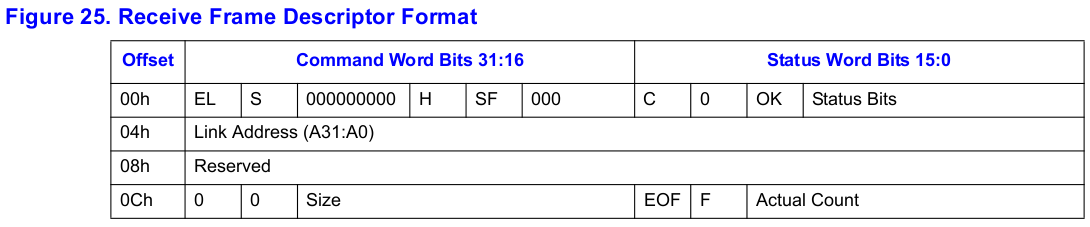
\includegraphics[scale=0.30]{/home/zhangchi/lab/report/rfd.png}
\end{figure}

这里控制字和状态字中需要我们注意的只有S和C两位,没有CMD。
\begin{itemize}
\item{如果S被设置成1,那么RU在接受完这个RFD的数据以后,挂起}
\item{如果C被设置成1,那么代表接收完成,注意\highlight{接收之前用户应该完成这个位的清除工作}}
\end{itemize}

前面的都和TCB是差不多的,但是下面的有两个场位是不同的:

\begin{itemize}
\item{Size: 表示data buffer的大小,在我们的数据中,数据包大小最大为1518,这个值在接收数据之前要\highlight{由用户来设置好}。}
\item{Actual Count: 如果C被置1表示接收完成,那么Actual Count表示的就是data buffer中总共的数据bytes数。这个是\highlight{由RU接收完以后填好}}
\end{itemize}

根据这些字段说明,我们把他们定义到头文件里方便后面使用和设置:

\begin{lstlisting}[style=ccode, title={\scriptsize \ttfamily \bfseries kern/e100.h}]
// Recieve Frame Descriptor Command
#define RFDF_EL         0x8000
#define RFDF_S          0x4000
#define RFDF_H          0x10
#define RFDF_SF         0x8


// Recieve Frame Descriptor Status
#define RFDS_C          0x8000
#define RFDS_OK         0x2000
#define RFDS_MASK       0x1fff


// Recieve Frame Descriptor Data
#define RFD_SIZE_MASK   0x3fff
#define RFD_AC_MASK     0x3fff
#define RFD_EOF         0x8000
#define RFD_F           0x4000
\end{lstlisting}

了解完RFD的结构,类似的,我们需要在其上面实现一个\highlight{支持多数据包等待接收的排队系统},同样也要注意两方面
\begin{enumerate}
\item{首先要记录的是当前RFA环状结构中哪些RFD是已经被RU收取完毕,\highlight{正等待被用户接收的},哪些是\highlight{可以被RU重新利用来接受新数据的}}
\item{其次要做好相应的S位设置,让RU在接收到不能接收的时候就停下来,不要让它将还没被用户接收的RFD覆盖了}
\end{enumerate}

\begin{lstlisting}[style=ccode, title={\scriptsize \ttfamily \bfseries kern/e100.h}]
#define RFD_MAXSIZE     1518
#define RFD_MAX_NUM     10

// Receive Frame Descriptor
struct rfd {
    volatile uint16_t rfd_status;
    uint16_t rfd_control;
    uint32_t rfd_link;

    uint32_t rfd_reserved;
    uint16_t rfd_actual_count;
    uint16_t rfd_size;

    char rfd_data[RFD_MAXSIZE];

    struct rfd *prev, *next;
    physaddr_t phy_addr;   
};

// Receive Frame Area
struct rfa {
    int rfd_avail;
    int rfd_wait;

    struct rfd *start;
    struct rfd *front, *rear;
};
\end{lstlisting}


struct rfd的结构没什么好说的,按照手册的规定设计即可,这里关键的是struct rfa,虽然和struct cbl的成员结构几乎一模一样,但是他们两者成员的意义是不一样的。

\begin{itemize}
\item{rfd\_avail: 表示当前有多少个闲置的RFD可以用来\highlight{接收RU新收到的数据}}
\item{rfd\_wait: 表示当前有多少个RFD正在处于\highlight{等待被用户接收}的状态}
\item{很明显上面两者相加应该等于所有RFD的总数,在这里应该是我们定义的RFD\_MAX\_NUM = 10}
\item{start: 所有RFD中的第一个RFD,用于开始的时候初始化RU用}
\item{front和rear: 表示当前\highlight{正在等待被用户接收}的RFD的起始和结尾}

\end{itemize}


那么这个系统是如何根据rfa中定义的结构工作的呢?

\begin{enumerate}
\item{初始的时候 front=start, rear=start$\rightarrow$prev,表示当前等待被用户接收的RFD队列为空,同时将start$\rightarrow$prev的Suspend控制位设成1,有两个目的:

\label{ruwork}

\begin{itemize}

\item{在第一次让RU开始执行START指令时,让RU可以一直接收数据直到最后一个RFD才停下。}
\item{一旦RU开始运行,保证任何时候队列里只有front$\rightarrow$prev的S位为1,即RU一直接受数据\highlight{直到front之前就要停止}}
\end{itemize}

并且rfd\_avail = RFD\_MAX\_NUM, rfd\_wait = 0}
\item{当用户需要收取一个数据包时,将front的内容取出,作为数据返回。并且清空front$\rightarrow$prev的S位,将front的S位置为1,表示该位置\highlight{可以让RU重新回收使用了}。做完以后front向后移动一个位置。同时增加rfd\_avail, 减少rfd\_wait}
\item{当确认数据包被RU接收完毕时,检查rear的后一个指向TCB的C状态是否为1,可以的话则将rear向后移动,同时减少rfd\_avail, 增加rfd\_wait}

\end{enumerate}


\vspace{2em}
\hrule
\vspace{2em}

好了RFA的结构了解完毕,现在我们可以考虑建立起这样的结构了:

\begin{lstlisting}[style=exercise]
|Exercise 8|. Construct a receive DMA ring and start the RU. If you use interrupts, make sure that 82559ER-generated interrupts are routed to your driver and are handled.
\end{lstlisting}

首先将RFA加入nic结构:

\begin{lstlisting}[style=ccode, title={\scriptsize \ttfamily \bfseries kern/e100.h}]
// Network Interface Card
struct nic {
    uint32_t io_base;
    uint32_t io_size;

    struct cbl cbl;
    struct rfa rfa;
};\end{lstlisting}

然后为RFA分配物理空间:


\begin{lstlisting}[style=ccode, title={\scriptsize \ttfamily \bfseries kern/e100.c: rfa\_alloc()}]
static void
rfa_alloc () {
    int i, r;
    struct Page *p;
    struct rfd *prevrfd = NULL;
    struct rfd *currrfd = NULL;

    // Allocate physical page for Control block
    for (i = 0; i < RFD_MAX_NUM; i++) {
        if ((r = page_alloc (&p)) != 0)
            panic ("rfa_init: run out of physical memory! %e\n", r);

        p -> pp_ref ++;
        memset (page2kva (p), 0, PGSIZE);

        currrfd = (struct rfd *)page2kva (p);
        currrfd->phy_addr = page2pa (p);
        currrfd->rfd_control = 0;
        currrfd->rfd_status = 0;
        currrfd->rfd_size = RFD_MAXSIZE;

        if (i == 0)
            nic.rfa.start = currrfd;
        else {
            prevrfd->rfd_link = currrfd->phy_addr;
            prevrfd->next = currrfd;
            currrfd->prev = prevrfd;
        }

        prevrfd = currrfd;
    }

    prevrfd->rfd_link = nic.rfa.start->phy_addr;
    nic.rfa.start->prev = prevrfd;
    prevrfd->next = nic.rfa.start;

    nic.rfa.rfd_avail = RFD_MAX_NUM;
    nic.rfa.rfd_wait = 0;

    nic.rfa.front = nic.rfa.start;
    nic.rfa.rear = nic.rfa.start->prev;
    nic.rfa.rear->rfd_control |= RFDF_S;
}

\end{lstlisting}

注意上面程序和\ref{cblalloc}的区别,因为RU一启动就开始等待接收数据,所以我们一开始就要设置好RFD的命令字、状态字和data buf大小等等,请关注18行到20行。最后将RFA中的末尾RFD的S位置成1。


\label{scbru}

然后是对RU的控制,前面在\ref{scb}介绍SCB时只介绍了针对CU的控制字和状态字,现在我们把RU的补充上来:

\begin{description}
\item[控制字]:\\
\begin{figure}[htp]
\centering
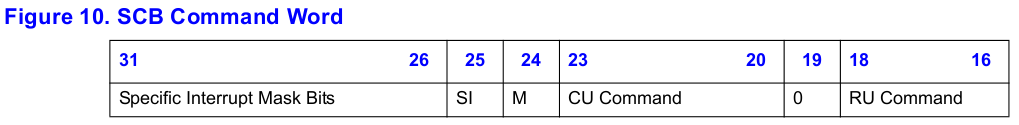
\includegraphics[scale=0.30]{/home/zhangchi/lab/report/scbcmd.png}
\end{figure}

RUC (RU Command): 这里对RU的控制命令有以下几种:

\begin{enumerate}
\item{000 NOP}
\item{001 RU Start}
\item{010 RU Resume}
\item{011 Receive DMA Redirect}
\item{100 RU Abort}
\item{101 Load Header Data Size (HDS)}
\item{110 Load RU Base}
\end{enumerate}

我们要用到的主要是\highlight{RU Start}和\highlight{RU Resume},把相应的设置场位定义到kern/e100.h中:

\begin{lstlisting}[style=ccode, title={\scriptsize \ttfamily \bfseries kern/e100.h}]
// RU Command Word
#define RUC_NOP         0x0
#define RUC_START       0x1
#define RUC_RESUME      0x2
#define RUC_REDIR       0x3
#define RUC_ABORT       0x4
#define RUC_LOADHDS     0x5
#define RUC_LOAD_BASE   0x6
\end{lstlisting}


\item[状态字]:\\
\begin{figure}[htp]
\centering
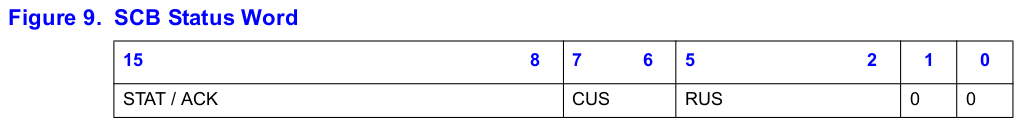
\includegraphics[scale=0.30]{/home/zhangchi/lab/report/scbstatus.png}
\end{figure}

RU的状态字主要可能有以下状态:

\begin{enumerate}
\item{0000: Idle}
\item{0001: Suspend}
\item{0010: No resources}
\item{0011: Reserved}
\end{enumerate}

我们只需要知道Suspend用于给出恢复命令时判断RU的当前状态,相关头文件定义:

\begin{lstlisting}[style=ccode, title={\scriptsize \ttfamily \bfseries kern/e100.h}]
// RU Status Word
#define RUS_MASK        0x3c
#define RUS_IDLE        0x0
#define RUS_SUSPEND     0x4
#define RUS_NORES       0x8
#define RUS_READY       0x10
\end{lstlisting}

\end{description}

\vspace{2em}
\hrule
\vspace{2em}

下面尝试初始化RFA。首先是两种对于RFA的操作:
\begin{itemize}
\item{第一种是确认其所在RFD的数据被RU接收完成}
\item{第二种是从队头取出一个数据准备返回给用户}
\end{itemize}

这两种操作的情况我们在前面\ref{ruwork}已经说过了。后面给出的程序中第一种操作对应\funcname{rfa\_validate()},第二种操作对应\funcname{rfa\_retrieve\_data()}。

为了保证我们后面编写系统调用的正确性,我们在初始化的时候就尽量对前面的RFA初始化以及指令操控作了一系列的测试,保证不要将错误在外层调用它时才显现出来,以免陷入混乱的调试。所以我们在程序中打印了一些消息用于查看:

\begin{lstlisting}[style=ccode, title={\scriptsize \ttfamily \bfseries kern/e100.c}]
static void
rfa_validate () 
{
    while (nic.rfa.rfd_avail > 0 && (nic.rfa.rear->next->rfd_status & RFDS_C) != 0) {
        nic.rfa.rear = nic.rfa.rear->next;

        nic.rfa.rfd_avail --;
        nic.rfa.rfd_wait ++;
        cprintf ("zhangchi: validate, avail = %d, wait = %d,   slot = %x\n", 
            nic.rfa.rfd_avail, nic.rfa.rfd_wait, nic.rfa.rear);
    }
}

static int
rfa_retrieve_data (char* data)
{
    if (nic.rfa.rfd_wait == 0)
        return -E_RFA_EMPTY;

    nic.rfa.rfd_avail ++;
    nic.rfa.rfd_wait --;
    cprintf ("zhangchi: retrieve, avail = %d, wait = %d,   slot = %x\n", 
        nic.rfa.rfd_avail, nic.rfa.rfd_wait, nic.rfa.front);

    nic.rfa.front->prev->rfd_control &= ~RFDF_S;
    nic.rfa.front->rfd_control = RFDF_S;
    nic.rfa.front->rfd_status = 0;

    int r = nic.rfa.front->rfd_actual_count & RFD_AC_MASK;
    memmove (data, nic.rfa.front->rfd_data, r);

    nic.rfa.front = nic.rfa.front->next;

    return r;
}\end{lstlisting}

其中\funcname{rfa\_retrieve\_data()} 接受一个buffer作为参数,如果当前RFA为空,那么返回一个负数错误码,否则将数据填入buffer后返回传输的数据字节数。

然后主过程是这么写的:

\begin{lstlisting}[style=ccode, title={\scriptsize \ttfamily \bfseries kern/e100.c: rfa\_init()}]
static void
rfa_init () 
{
    cprintf ("\n\nRFA Initialization started! \n");
    rfa_alloc ();

    outl(nic.io_base + CSR_GP, nic.rfa.front->phy_addr);
    e100_exec_cmd (CSR_COMMAND, RUC_START); 

    while (nic.rfa.rfd_avail > 0)
        rfa_validate ();

    int scb_status = inb(nic.io_base + CSR_STATUS);
    cprintf ("zhangchi: rfd slot is full, current RU state = %02x\n", 
        scb_status & RUS_MASK);

    char s[1518];
    while (rfa_retrieve_data (s) >= 0);

    e100_exec_cmd (CSR_COMMAND, RUC_RESUME);

    while (nic.rfa.rfd_avail > 0)
        rfa_validate ();
}
\end{lstlisting}

可以看到在为RFA分配物理内存以后,马上会进行一系列的测试:

\begin{enumerate}
\item{第7行,给RU发送START命令,使其开始接收数据包,因为初始化的时候只有最后一个RFD设置了S标志,所以开始以后只有当RU将所有RFD都接收了数据才会停下来}
\item{第10行,不断检查系统中可用RFD的个数,当其减少到0的时候,就证明整个RFA已经被RU收到的数据塞满了。在\funcname{rfa\_validate()}检查过程中一旦发现有新收到的数据,将会打印出一条validate信息}
\item{第18行,被塞满以后数据应该被发送到用户,这里我们只是单纯的把数据提取出来,不作处理。\funcname{rfa\_retrieve\_data()} 执行过程中也会打印出一条信息。
}
\item{第20行,开始让RU继续接收数据}
\end{enumerate}

测试的时候我们使用make qemu QEMUEXTRA="-debug-e100 -pcap slirp.cap"启动JOS,那么初始JOS应该会停滞在第10行轮询检查可用RFD的个数,那么这个时候如果开始给它发消息,就会有相应信息打印出来了,新开一个terminal使用make nc-7命令即可向网卡发送数据包,下面是我们得到的输出(为了打印长度的考虑,我把RFD\_MAX\_NUM改成了4,使我们能更快看到程序执行到边界条件)。


\begin{lstlisting}[style=console, basicstyle=\tiny\color{green}\ttfamily\bfseries]
RFA Initialization started! 
EE100	eepro100_write_pointer  val=0x040b1000
EE100	eepro100_write1         addr=Command/Status+2 val=0x01
EE100	eepro100_ru_command     val=0x01 (rx start)
EE100	eepro100_read1          addr=Command/Status+2 val=0x00
EE100	nic_can_receive         0x8adc008
EE100	nic_receive             0x8adc008 received broadcast, len=42
EE100	nic_receive             command 0x0000, link 0x040b0000, addr 0x00000000, size 1518
zhangchi: validate, avail = 3, wait = 1,   slot = f40b1000
EE100	nic_can_receive         0x8adc008
EE100	nic_receive             0x8adc008 received broadcast, len=42
EE100	nic_receive             command 0x0000, link 0x040af000, addr 0x00000000, size 1518
zhangchi: validate, avail = 2, wait = 2,   slot = f40b0000
EE100	nic_can_receive         0x8adc008
EE100	nic_receive             0x8adc008 received broadcast, len=42
EE100	nic_receive             command 0x0000, link 0x040ae000, addr 0x00000000, size 1518
zhangchi: validate, avail = 1, wait = 3,   slot = f40af000
EE100	nic_can_receive         0x8adc008
EE100	nic_receive             0x8adc008 received broadcast, len=42
EE100	nic_receive             command 0x4000, link 0x040b1000, addr 0x00000000, size 1518
zhangchi: validate, avail = 0, wait = 4,   slot = f40ae000
EE100	eepro100_read1          addr=Command/Status+0 val=0x44
zhangchi: rfd slot is full, current RU state = 04
zhangchi: retrieve, avail = 1, wait = 3,   slot = f40b1000
zhangchi: retrieve, avail = 2, wait = 2,   slot = f40b0000
zhangchi: retrieve, avail = 3, wait = 1,   slot = f40af000
zhangchi: retrieve, avail = 4, wait = 0,   slot = f40ae000
EE100	eepro100_write1         addr=Command/Status+2 val=0x02
EE100	eepro100_read1          addr=Command/Status+2 val=0x00
EE100	nic_can_receive         0x8adc008
EE100	nic_receive             0x8adc008 received broadcast, len=42
EE100	nic_receive             command 0x0000, link 0x040b0000, addr 0x00000000, size 1518
zhangchi: validate, avail = 3, wait = 1,   slot = f40b1000
EE100	nic_can_receive         0x8adc008
EE100	nic_receive             0x8adc008 received broadcast, len=42
EE100	nic_receive             command 0x0000, link 0x040af000, addr 0x00000000, size 1518
zhangchi: validate, avail = 2, wait = 2,   slot = f40b0000
EE100	nic_can_receive         0x8adc008
EE100	nic_receive             0x8adc008 received broadcast, len=42
EE100	nic_receive             command 0x0000, link 0x040ae000, addr 0x00000000, size 1518
zhangchi: validate, avail = 1, wait = 3,   slot = f40af000
\end{lstlisting}

可以看到输出是符合我们的预期的,通过slot可以看到每次操作的RFD编号,可以观察RU操作这些RFD的顺序。测试成功以后,我们需要将初始化改回来:

\begin{lstlisting}[style=ccode, title={\scriptsize \ttfamily \bfseries kern/e100.c: rfa\_init()}]
static void
rfa_init () 
{
    rfa_alloc ();

    outl(nic.io_base + CSR_GP, nic.rfa.front->phy_addr);
    e100_exec_cmd (CSR_COMMAND, RUC_START); 
}
\end{lstlisting}

实验很顺利,可以考虑编写给系统调用的接口了:
\newpage

\begin{lstlisting}[style=exercise]
|Exercise 9|. Create a system call for receiving packets. As described in the Device Driver Organization section, the system call will read a packet out of the receive DMA ring, mark the DMA buffer as empty (so that the E100 can reuse it), resume the RU if necessary, and pass the packet to the calling user environment.
\end{lstlisting}

我设计的接口如下:



\begin{lstlisting}[style=ccode, title={\scriptsize \ttfamily \bfseries kern/e100.c: e100\_receive()}]
int 
e100_receive (char *data)
{
    rfa_validate ();

    if (nic.rfa.rfd_wait == 0)
        return -E_RFA_EMPTY;

    int r = rfa_retrieve_data (data);
    
    int scb_status = inb(nic.io_base + CSR_STATUS);
    if ((scb_status & RUS_MASK) == RUS_SUSPEND)
        e100_exec_cmd (CSR_COMMAND, RUC_RESUME); 

    return r;
}
\end{lstlisting}

如果没有数据可以获取,返回负数错误,否则将数据填入data代表的buffer,然后将数据的字节数作为返回值返回。

记得修改相关代码将系统调用安装到JOS中去。


\subsection{Receiving Packets: Network Server}



\begin{lstlisting}[style=exercise]
|Exercise 10|. Implement net/input.c.
\end{lstlisting}

这个Exercise是我本次实验花费的时间最多的地方之一,为什么,可以看看我的代码:

\begin{lstlisting}[style=ccode, title={\scriptsize \ttfamily \bfseries net/input.c}]
#include "ns.h"
#include <inc/lib.h>

extern union Nsipc nsipcbuf;

void
input(envid_t ns_envid)
{
    binaryname = "ns_input";

    while (1) {
        while ((nsipcbuf.pkt.jp_len 
            = sys_net_try_recv (nsipcbuf.pkt.jp_data)) < 0);

        ipc_send(ns_envid, NSREQ_INPUT, &nsipcbuf, PTE_U|PTE_W|PTE_P);     
    }
}
\end{lstlisting}

这段代码在测试的时候发现make grade在testinput死都不过,于是我尝试自己单独运行testinput, 在grade-lab6.sh中可以看到testinput是这么调用的:

\begin{lstlisting}[style=console]
runtest1 -tag "testinput [5 packets]" -dir net testinput -DTEST_NO_NS \
	-check check_testinput 5
\end{lstlisting}

注意DTEST\_NO\_NS是不启动网络服务器的宏,这就让我很纳闷了,如果不启动的话怎么测试Input和Output模块的?结果查看了一下net/testinput.c代码后才发现,它自己在进程中创建了Input环境和Output环境,单独对这两个模块进行测试:

\begin{lstlisting}[style=ccode, title={\scriptsize \ttfamily \bfseries kern/e100.c}]
void
umain(void)
{
	envid_t ns_envid = sys_getenvid();
	int i, r;

	binaryname = "testinput";

	output_envid = fork();
	if (output_envid < 0)
		panic("error forking");
	else if (output_envid == 0) {
		output(ns_envid);
		return;
	}

	input_envid = fork();
	if (input_envid < 0)
		panic("error forking");
	else if (input_envid == 0) {
		input(ns_envid);
		return;
	}

	cprintf("Sending ARP announcement...\n");
	announce();

	cprintf("Waiting for packets...\n");
	while (1) {
		envid_t whom;
		int perm;

		int32_t req = ipc_recv((int32_t *)&whom, pkt, &perm);
		if (req < 0)
			panic("ipc_recv: %e", req);
		if (whom != input_envid)
			panic("IPC from unexpected environment %08x", whom);
		if (req != NSREQ_INPUT)
			panic("Unexpected IPC %d", req);

		hexdump("input: ", pkt->jp_data, pkt->jp_len);
		cprintf("\n");
	}
}
\end{lstlisting}

所以单独运行testinput就只需要启动testinput进程就可以了,NS和FS都可以不用启动,反正也没有用到,即把kern/init.c的创建进程一段改成:

\begin{lstlisting}[style=ccode, title={\scriptsize \ttfamily \bfseries kern/init.c: i386\_init()}]
	// Should always have an idle process as first one.
	ENV_CREATE(user_idle);

	// Start fs.
	//ENV_CREATE(fs_fs);


#if !defined(TEST_NO_NS)
	//Start ns.
        //ENV_CREATE(net_ns);
#endif

#if defined(TEST)
	// Don't touch -- used by grading script!
	ENV_CREATE2(TEST, TESTSIZE);
#else
	// Touch all you want.
	ENV_CREATE(net_testinput);
	// ENV_CREATE(user_echosrv);
	// ENV_CREATE(user_httpd);
#endif // TEST*

	// Schedule and run the first user environment!

        sched_yield ();
\end{lstlisting}

然后make qemu发现出错了,内核地址错误:

\begin{lstlisting}[style=console]
Sending ARP announcement...
Waiting for packets...
TRAP frame at 0xefbffecc
  edi  0x00806004
  esi  0xf40b1010
  ebp  0xefbfff10
  oesp 0xefbffeec
  ebx  0x0000002a
  edx  0x0000000a
  ecx  0x0000002a
  eax  0x00806004
  es   0x----0010
  ds   0x----0010
  trap 0x0000000e Page Fault
  err  0x00000003
  eip  0xf0105b14
  cs   0x----0008
  flag 0x00003002
  esp  0xf0286208
  ss   0x----6004
kernel panic at kern/trap.c:313: kernel-mode page faults
Welcome to the JOS kernel monitor!
Type 'help' for a list of commands.
\end{lstlisting}

很奇怪,然后选择打印栈轨迹查看是从哪里出错的:

\begin{lstlisting}[style=console]
Welcome to the JOS kernel monitor!
Type 'help' for a list of commands.
K> backtrace
Stack backtrace:
  ebp efbffdc0  eip f010092a  args 00000001 efbffdd8 00000000 efbffe64 f0285d60
         kern/monitor.c:419: monitor+274
  ebp efbffe30  eip f01000e2  args 00000000 efbffe64 00000139 00000008 efbffecc
         kern/init.c:112: _panic+93
  ebp efbffe50  eip f01041f8  args f01086c0 00000139 f01086a8 00000008 00000000
         kern/trap.c:356: page_fault_handler+63
  ebp efbffe90  eip f01043d5  args efbffecc 00806000 efbffed0 f0103992 efbffef4
         kern/trap.c:232: trap+198
  ebp efbffec0  eip f0104582  args efbffecc 00806004 f40b1010 efbfff10 efbffeec
         kern/trapentry.S:103: <unknown>+0
  ebp efbfff10  eip f0106205  args 00806004 f40b1010 0000002a 007ff000 00000000
         kern/e100.c:328: e100_receive+196
  ebp efbfff30  eip f0104c1c  args 00806004 f02b8564 00807000 00000007 f02b9174
         kern/syscall.c:593: syscall+1535
  ebp efbfff80  eip f0104416  args 00000010 00806004 00000000 00000000 00000000
         kern/trap.c:248: trap+263
  ebp efbfffb0  eip f0104582  args efbfffbc 00000000 00000000 eebfdef0 efbfffdc
         kern/trapentry.S:103: <unknown>+0
  ebp eebfdef0  eip 0080050a  args 00806004 00000000 00000000 00001001 00001001
         <unknown>:0: <unknown>+0
  ebp eebfdf10  eip 008000ce  args 00001001 00000000 00000000 00000000 00000000
         <unknown>:0: <unknown>+0
  ebp eebfdfd0  eip 00800614  args 00000000 00000000 00000000 00000000 00000000
         <unknown>:0: <unknown>+0
\end{lstlisting}

看到其中出现了kern/e100.c:328 e100\_receive的信息,然后去源文件找到这行代码:

\begin{lstlisting}[style=ccode, firstnumber=323, title={\scriptsize \ttfamily \bfseries kern/e100.c: e100\_receive()}]
    nic.rfa.front->prev->rfd_control &= ~RFDF_S;
    nic.rfa.front->rfd_control = RFDF_S;
    nic.rfa.front->rfd_status = 0;

    int r = nic.rfa.front->rfd_actual_count & RFD_AC_MASK;
    memmove (data, nic.rfa.front->rfd_data, r);

    nic.rfa.front = nic.rfa.front->next;

    return r;
\end{lstlisting}

328行是memmove,也就是说往data里写入数据的时候出错了,data是input系统调用的传入参数,最外层的时候应该是由net/input.c中调用的:


\begin{lstlisting}[style=ccode, title={\scriptsize \ttfamily \bfseries net/input.c}]
#include "ns.h"
#include <inc/lib.h>

extern union Nsipc nsipcbuf;

void
input(envid_t ns_envid)
{
    binaryname = "ns_input";

    while (1) {
        while ((nsipcbuf.pkt.jp_len 
            = sys_net_try_recv (nsipcbuf.pkt.jp_data)) < 0);

        ipc_send(ns_envid, NSREQ_INPUT, &nsipcbuf, PTE_U|PTE_W|PTE_P);     
    }
}
\end{lstlisting}

第12行的sys\_net\_try\_recv 就是调用的 e100\_receive (),为什么写入 nsipcbuf.pkt.jp\_data会错误呢?我百思不得其解,直到\highlight{张顺廷}湿胸提醒我才明白过来,Input和Output都是由testinput这个进程fork出来的,因此对于nsipcbuf这样的数据,在他们的地址中都是\highlight{COW页}。

如果按照我这样的调用方法传入调用系统调用,那么向nsipcbuf中写入值的时候由于是处在内核态,内核态没有COW恢复机制,所以就发生了内核页错误了。COW恢复只可能是在用户态程序中进行写入时才有可能发生,即只有在Input本身向nsipcbuf写入数据,才有可能恢复。

所以处理的办法是,在Input环境中开一片buf专门用于存储从系统调用 \funcname{ sys\_net\_try\_recv() } 接受来的数据,然后在接收以后再复制给 nsipcbuf.pkt.jp\_data,修改后的Input如下:

\begin{lstlisting}[style=ccode, title={\scriptsize \ttfamily \bfseries net/input.c}]
#include "ns.h"
#include <inc/lib.h>

extern union Nsipc nsipcbuf;

void
input(envid_t ns_envid)
{
    binaryname = "ns_input";
    char buf[1518];
    int len;

    while (1) {
        while ((len = sys_net_try_recv (buf)) < 0);

        nsipcbuf.pkt.jp_len = len;
        memmove ((void*) nsipcbuf.pkt.jp_data, (void *) buf, len);

        ipc_send(ns_envid, NSREQ_INPUT, &nsipcbuf, PTE_U|PTE_W|PTE_P);     
    }
}
\end{lstlisting}

修改以后再次测试,出现了很奇怪的现象:

\begin{lstlisting}[style=console]
testinput [5 packets]: WRONG, receiving packet 001/5 (5.0s)
expected input: 0030   2030 3031 0a
got      input: 0030   2030 3032 0a
testinput [100 packets]: WRONG, receiving packet 001/100 (5.2s)
expected input: 0030   2030 3031 0a
got      input: 0030   2030 3032 0a
tcp echo server [echosrv]: OK (5.0s)
\end{lstlisting}

echosvr过了,但是testinput还是不过,而且跟答案的差距还非常小,在怎么检查都查不出的情况下,我通过比对张磊同学的代码,发现了我忘记看他提示中的一句话:

\begin{lstlisting}[style=challenge]
    // LAB 6: Your code here:
    // 	- read a packet from the device driver
    //	- send it to the network server
    // Hint: When you IPC a page to the network server, it will be
    // reading from it for a while, so don't immediately receive
    // another packet in to the same physical page.
\end{lstlisting}

即会有这样的情况,Input将数据放入nsipcbuf中传给NS,NS处理这些数据需要一些时间。因为Input 是轮询查询网卡是不是有新数据的,所以可能在NS还没处理完的时候就利用原来的页面装进了新收到的数据,准备发给NS,这个时候就悲剧了,原来的数据被刷新了。

张磊的做法是每次把nsipcbuf以ipc发送给NS以后,进行一次 \funcname{sys\_yield()} 我也这么试了,让我很郁闷,他进行一次就可以了,我一定要yield三次才可以。其实事实上yield多少次都不安全,因为没法知道网络服务器端什么时候才读完所有的数据,允许Input可以在nsipcbuf上写新的东西。

所以我的想法是应该让网络服务器接受和处理完毕以后,向Input发送一条消息,通知他可以继续收数据。但是具体服务器代码我没有看,所以也无所谓改不改了。


\subsection{The Web Server}

\begin{lstlisting}[style=exercise]
|Exercise 11|. The web server is missing the code that deals with sending the contents of a file back to the client. Finish the web server by implementing send_file and send_data.
\end{lstlisting}

这段程序主要是查询文件系统中关于Socket的用法,以及将文件读取连接后输出,都不难,直接贴代码了:

\begin{lstlisting}[style=ccode, title={\scriptsize \ttfamily \bfseries user/httpd.c: send\_file()}]
static int
send_file(struct http_request *req)
{
	int r;
	off_t file_size = -1;
	int fd;

	// open the requested url for reading
	// if the file does not exist, send a 404 error using send_error
	// if the file is a directory, send a 404 error using send_error
	// set file_size to the size of the file

	// LAB 6: Your code here.
 	char path[MAXPATHLEN];
	struct Stat stat;

	memmove(path, req->url, strlen(req->url));

        if ((fd = open(path, O_RDONLY)) < 0) {
            send_error(req, 404);
            goto end;
        }

        if ((r = fstat(fd, &stat)) < 0) {
            goto end;
        }

        if (stat.st_isdir) {
            send_error(req, 404);
            goto end;
        }
 
        file_size = stat.st_size;


	if ((r = send_header(req, 200)) < 0)
		goto end;

	if ((r = send_size(req, file_size)) < 0)
		goto end;

	if ((r = send_content_type(req)) < 0)
		goto end;

	if ((r = send_header_fin(req)) < 0)
		goto end;

	r = send_data(req, fd);

end:
	close(fd);
	return r;
}
\end{lstlisting}

还有

\begin{lstlisting}[style=ccode, title={\scriptsize \ttfamily \bfseries user/httpd.c: send\_data()}]
static int
send_data(struct http_request *req, int fd)
{
	// LAB 6: Your code here.
	char *buff = malloc(1520 + 10);
	struct Stat stat;
	int size, r;

	if (fstat(fd, &stat) < 0) {
		return 0;
	}
	size = stat.st_size;

	if (size > 1520 + 10)
		return 0;
	if ((r = readn(fd, buff, stat.st_size)) < 0) {
		return 0;
	}
	if (write(req->sock, buff, stat.st_size) != stat.st_size)
		cprintf("Failed to send the file\n");

	return 0;
}
\end{lstlisting}

\vspace{3em}

到这里Lab6终于完全结束了!真的太消耗人了。

\clearpage

\end{CJK*}
\end{document}
	

e